
\documentclass[10pt, a4paper]{article}

\setlength{\textheight}{24.5cm}
\setlength{\topmargin}{-18mm}
\setlength{\textwidth}{16cm}
\setlength{\oddsidemargin}{0mm} % marge gauche (im)paire = 1in. + x1mm
%\setlength{\evensidemargin}{-5mm} % book : marge gauche paire = 1in. + x2mm

\setlength{\fboxsep}{1mm}
\setlength{\unitlength}{1mm}

\usepackage{fancyhdr}
\usepackage{graphicx}
\usepackage{amsmath}  
\usepackage{latexsym}
\usepackage[francais]{babel}
%\usepackage[latin1]{inputenc}
\usepackage[utf8]{inputenc}
\usepackage{natbib}
\usepackage{color}
\usepackage{textcomp}
 \usepackage{lscape}
\usepackage{accents}

\input{./TD_fluides.macros}
%\usepackage{cancel}
% Style des vecteurs : fleche ou gras ?

%\newcommand{\myvec}[1]{\boldsymbol{#1}}
\newcommand{\myvec}[1]{\vec{#1}}

\newcommand{\mytensor}[1]{\accentset{\Rightarrow}{#1}} % needs \usepackage{accents}

%---------------------------
% Operateurs differentiels :
%---------------------------

\newcommand{\divergence}{\mbox{\rm div}\,}

\newcommand{\gradient}{\myvec{\mbox{\rm gra}}\mbox{\rm d}}
% \newcommand{\gradient}{\mathbf{grad}\,}
% \newcommand{\ggradient}{\stackrel{\Rightarrow}{\mbox{gra}}\!\!\!\,\mbox{d}\,}
\newcommand{\ggradient}{\accentset{\Rightarrow}{\mbox{\rm gra}}\mbox{\rm d}\!}

%\renewcommand{\dot}[1]{\accentset{\hbox{\huge .}}{#1}}
\newcommand{\mydot}[1]{\accentset{\centerdot}{#1}}

\newcommand{\rot}{\vec{\mbox{\rm ro}}\mbox{\rm t}\,}
%\newcommand{\rot}{\mathbf{rot}\,}

% \newcommand{\vnabla}{\vec{\nabla}}
\newcommand{\vnabla}{\boldsymbol{\nabla}}

% Fonctions speciales:

\newcommand{\besselj}[1]{\mbox{J}_{#1}}
\newcommand{\besselk}[1]{\mbox{K}_{#1}}
\newcommand{\bessely}[1]{\mbox{Y}_{#1}}
\newcommand{\besseli}[1]{\mbox{I}_{#1}}

% Vecteurs, tenseurs et torseurs:

\newcommand{\ex}{\mathbf{e}_{x}}
\newcommand{\ey}{\mathbf{e}_{y}}
\newcommand{\ez}{\mathbf{e}_{z}}

\newcommand{\er}{\mathbf{e}_{r}}
\newcommand{\erho}{\mathbf{e}_{\rho}}
\newcommand{\ephi}{\mathbf{e}_{\varphi}}
\newcommand{\etheta}{\mathbf{e}_{\theta}}

%\newcommand{\tensor}[1]{\stackrel{\Rightarrow}{#1}}
\newcommand{\tensor}[1]{\mbox{\sl \textbf{#1}}}
\newcommand{\torseur}[4]{
   \!\!\!\! \left . \begin{array}{c} \\ \\ _#1 \end{array} \!\!\!
   \right \{ \!\!\!
   \begin{array}{#4} #2 \\ \\ #3 \end{array}}

% Integrales multiples:

\newcommand{\odblint}[1]{\int\!\!\!\!\!\int_{#1} \hskip -7mm \bigcirc \;}
\newcommand{\dblint}{\int\!\!\!\!\!\int}
\newcommand{\tplint}{\int\!\!\!\!\!\int\!\!\!\!\!\int}

% Fractions:

\renewcommand{\dfrac}[2]{\displaystyle \frac{#1}{#2}}

% Derivees ordinaires et partielles:

\newcommand{\dpdt}[1]{\dfrac{\partial #1}{\partial t}}
\newcommand{\dpdx}[1]{\dfrac{\partial #1}{\partial x}}
\newcommand{\dpdy}[1]{\dfrac{\partial #1}{\partial y}}
\newcommand{\dpdz}[1]{\dfrac{\partial #1}{\partial z}}

\newcommand{\ddpdt}[1]{\dfrac{\partial^2 #1}{\partial t^2}}
\newcommand{\ddpdx}[1]{\dfrac{\partial^2 #1}{\partial x^2}}
\newcommand{\ddpdy}[1]{\dfrac{\partial^2 #1}{\partial y^2}}
\newcommand{\ddpdz}[1]{\dfrac{\partial^2 #1}{\partial z^2}}

\newcommand{\dpdr}[1]{\dfrac{\partial #1}{\partial r}}
\newcommand{\dpdrho}[1]{\dfrac{\partial #1}{\partial \rho}}
\newcommand{\dpdphi}[1]{\dfrac{\partial #1}{\partial \varphi}}
\newcommand{\dpdtheta}[1]{\dfrac{\partial #1}{\partial \theta}}

\newcommand{\ddpdr}[1]{\dfrac{\partial^2 #1}{\partial r^2}}
\newcommand{\ddpdrho}[1]{\dfrac{\partial^2 #1}{\partial \rho^2}}
\newcommand{\ddpdphi}[1]{\dfrac{\partial^2 #1}{\partial \varphi^2}}
\newcommand{\ddpdtheta}[1]{\dfrac{\partial ^2#1}{\partial \theta^2}}

\newcommand{\ddt}[1]{\dfrac{d #1}{dt}}
\newcommand{\ddx}[1]{\dfrac{d #1}{dx}}
\newcommand{\ddy}[1]{\dfrac{d #1}{dy}}
\newcommand{\ddz}[1]{\dfrac{d #1}{dz}}
\newcommand{\ddr}[1]{\dfrac{d #1}{dr}}

\newcommand{\ddtref}[2]{\dfrac{d #1}{dt}_{\! | #2 }}
\newcommand{\dpdtref}[3]{\dfrac{\partial #1}{\partial #2}_{\! | #3 }}

% Misc:

\newcommand{\mycaption}[1]{\caption{\sl #1}}

\newcommand{\ligne}[1]{\hrule height #1\linethickness \hfill}

\newcommand{\thickline}[2]{\linethickness{#1} \line(1, 0){#2}}

\newcommand{\myline}{\noindent\underline{\hspace{\textwidth}}}
\newcommand{\mysection}[1]{\vskip 0.5cm \section{#1}\vskip -1.4cm 
   \myline \vskip 0.4cm \myline \bigskip}

\newcommand{\etal}{\textit{et al.}}

\newcommand{\varray}[1]{\renewcommand{\arraystretch}{#1}}

\newcommand{\puissance}[1]{^{\mbox{\footnotesize #1}}}
\newcommand{\indice}[1]{_{\mbox{\footnotesize #1}}}

%---------------------------------------------------------------------
% New environments:
%---------------------------------------------------------------------

\newcounter{MyEnumCounter}
\newcounter{MySaveCounter}
\newenvironment{MyEnum}{%
  \begin{list}{\arabic{MyEnumCounter}.}{\usecounter{MyEnumCounter}%
  \setcounter{MyEnumCounter}{\value{MySaveCounter}}}
  }{%
  \setcounter{MySaveCounter}{\value{MyEnumCounter}}\end{list}%
}
\newcommand{\MyEnumReset}{\setcounter{MySaveCounter}{0}}

\newenvironment{deuxcols}{\begin{tabular}{lr} \hspace*{-9.7mm}}{\end{tabular}}

\newenvironment{dem}{\noindent %
   \begin{tabular}{||l} \textsl{D\'emonstration :} \\ % 
   \begin{minipage}{15.5cm} \footnotesize} %
   {\end{minipage}\end{tabular}}

\newenvironment{abst}{\begin{quotation}\sl}{\end{quotation}}

\newenvironment{eqnbox}{\begin{equation}\begin{array}{|c|}  \hline \\ 
   \displaystyle}{\\ \\ \hline \end{array} \end{equation}}

\newcommand{\myprime}{\ \!'}

% JFM symbols:

\DeclareMathSymbol{\varGamma}{\mathord}{letters}{"00}
\DeclareMathSymbol{\varDelta}{\mathord}{letters}{"01}
\DeclareMathSymbol{\varTheta}{\mathord}{letters}{"02}
\DeclareMathSymbol{\varLambda}{\mathord}{letters}{"03}
\DeclareMathSymbol{\varXi}{\mathord}{letters}{"04}
\DeclareMathSymbol{\varPi}{\mathord}{letters}{"05}
\DeclareMathSymbol{\varSigma}{\mathord}{letters}{"06}
\DeclareMathSymbol{\varUpsilon}{\mathord}{letters}{"07}
\DeclareMathSymbol{\varPhi}{\mathord}{letters}{"08}
\DeclareMathSymbol{\varPsi}{\mathord}{letters}{"09}
\DeclareMathSymbol{\varOmega}{\mathord}{letters}{"0A}

% ---------------------------------------------------------------------
% MISC SYMBOLS :
% ---------------------------------------------------------------------

\font\SY=msam10 
\def\carreblanc{\hbox{\SY \char'3}}
\def\carrenoir{\hbox{\SY \char'4}}
\def\diamblanc{\hbox{\SY \char'6}}
\def\diamnoir{\hbox{\SY \char'7}}
\def\triblancright{\hbox{\SY \char'102}}
\def\triblancleft{\hbox{\SY \char'103}}
\def\triblancup{\hbox{\SY \char'115}}
\def\triblancdown{\hbox{\SY \char'117}}
\def\trinoirright{\hbox{\SY \char'111}}
\def\trinoirleft{\hbox{\SY \char'112}}
\def\trinoirup{\hbox{\SY \char'116}}
\def\trinoirdown{\hbox{\SY \char'110}}
\def\rondblanc{\hbox{\scriptsize $\bigcirc$}}
\def\rondnoir{\hbox{\LARGE $\bullet$}}

\font\BB=msbm10 scaled 1095
\def\setr{\hbox{\BB R}}
\def\setc{\hbox{\BB C}}
\def\setn{\hbox{\BB N}}
\def\setz{\hbox{\BB Z}}

% Pour enlever la numerotation des pages de la table des matieres:

%%%% debut macro, a placer dans preambule %%%%
\makeatletter
\def\addcontentsline@toc#1#2#3{%
   \addtocontents{#1}{\protect\thispagestyle{empty}}%
   \addtocontents{#1}{\protect\contentsline{#2}{#3}{\thepage}}}
\def\addcontentsline#1#2#3{%
  \expandafter\@ifundefined{addcontentsline@#1}%
  {\addtocontents{#1}{\protect\contentsline{#2}{#3}{\thepage}}}
  {\csname addcontentsline@#1\endcsname{#1}{#2}{#3}}}
\makeatother
%%%% fin macro %%%%

\newcommand{\titre}[1]{ %
  \medskip \noindent \underline{\makebox[\textwidth][l]{\textbf{#1}\textcolor{white}{pl}}}}% \\}

\newcommand{\sstitre}[1]{ %
  \bigskip \centerline{\textbf{#1}} \smallskip}

\def\draft{\overfullrule 5pt} % The \draft command marks the overful boxes

\def\indentlist{\list%
        {}{\labelwidth 0pt \leftmargin 3\labelsep}}
\let\endindentlist\endlist \relax

\def\datelist{\list%
        {}{\settowidth\labelwidth{[2001/02 :]}
        \leftmargin\labelwidth
        \advance\leftmargin\labelsep}
}
\let\enddatelist\endlist \relax

\def\longuelist{\list%
        {}{\settowidth\labelwidth{[Etablissement :]}
        \leftmargin\labelwidth
        \advance\leftmargin\labelsep}
}
\let\endlonguelist\endlist \relax

\def\shortlist{\list%
        {}{\settowidth\labelwidth{$\bullet$}
        \leftmargin\labelwidth
        \advance\leftmargin\labelsep}
}
\let\endshortlist\endlist \relax




\newcommand{\e}{\mathrm{e}}   
\newcommand{\dd}{\textrm d}      
\newcommand{\im}{\mathrm{i}}
\newcommand{\dpa}[2]{\frac {\partial #1} {\partial #2}}   
\newcommand{\ddpa}[2]{\frac {\partial^{2} #1} {\partial #2 ^{2}}}   
\newcommand{\dto}[2]{\frac {{\textrm d} #1} {{\textrm d} #2}}   
\newcommand{\ddto}[2]{\frac {{\textrm d}^{2} #1} {{\textrm d} #2 ^{2}}}
\newcommand{\mytensor}[1]{\accentset{=}{#1}} % needs \usepackage{accents}

\newcommand{\exofacile}{$^\star$}
%\newcommand{\exonormal}{$^\star$$^\star$}
\newcommand{\exonormal}{$^\star$}
%\newcommand{\exodifficile}{$^\star$$^\star$$^\star$}
\newcommand{\exodifficile}{$^\star$$^\star$}

\usepackage[final]{pdfpages}

\newcommand{\Archives}[1]{}
\newcommand{\comment}[1]{}

\newcommand{\rep}[1]{}

\graphicspath{{./Figures/}{./Figures_Fluides_L2/}}

%%%%%%%%%%%%%%%%%%%%%%%%%%%%%%%%%%%%%%%%%%%%%%%%%%%%%%%%%%%%%%%%%%%%%%%%%%%%%%%%%%%%%%%%%%%%%%%%%%%
\begin{document}                                          
%%%%%%%%%%%%%%%%%%%%%%%%%%%%%%%%%%%%%%%%%%%%%%%%%%%%%%%%%%%%%%%%%%%%%%%%%%%%%%%%%%%%%%%%%%%%%%%%%%%

\begin{titlepage}

\noindent
\textsc{Universit\'e Toulouse 3 -- Paul Sabatier \hfill Ann\'ee universitaire 2018-2019}
\\
\textsc{L3 M\'ecanique \hfill M\'ecanique des fluides}

\vspace{1cm}

\begin{center}
  \setlength{\unitlength}{1mm}
  \hrule height 1mm
  \vspace{6mm}
  \textbf{\LARGE Exercices et probl\`emes -- 2ème partie}
  \\ \vspace{5mm}
  \hrule height 1mm
  \vspace{2cm}
  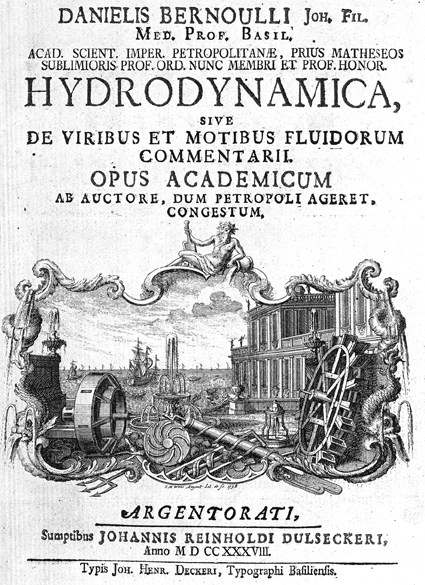
\includegraphics[width=10cm]{bernoulli}
\end{center}

\vfill

\begin{flushright}
  \large{\textsl{Equipe p\'edagogique : \\
      D. Fabre, M. Zagzoule, F. Moulin}}
\end{flushright}

\end{titlepage}

%%%%%%%%%%%%%%%%%%%%%%%%%%%%%%%%%%%%%%%%%%%%%%%%%%%%%%%%%%%%%%%%%%%%%%%%%%%%%%%%%%%%%%%%%%%%%%%%%%%
\setcounter{secnumdepth}{2}
\tableofcontents
%%%%%%%%%%%%%%%%%%%%%%%%%%%%%%%%%%%%%%%%%%%%%%%%%%%%%%%%%%%%%%%%%%%%%%%%%%%%%%%%%%%%%%%%%%%%%%%%%%%

% !TEX root = TD_fluides_part2_2018.tex

\setcounter{section}{6}

%\section{Ecoulements Inertiels II : Ecoulements potentiels}


\section{Ecoulements Inertiels I }


\setcounter{subsection}{-1}


\subsection{Vidange d'un réservoir}

{\em Exercice préparatoire ; énoncé et correction détaillée sur moodle}

%--------------------------------------------------------------------------------------------------
\subsection{Force exerc\'ee par un jet sur une plaque}
%--------------------------------------------------------------------------------------------------

\begin{figure}[hbtp]
  \begin{center}
    \setlength{\unitlength}{1mm}
    \begin{picture}(80, 60)(0, 0)
      \put(10, 0){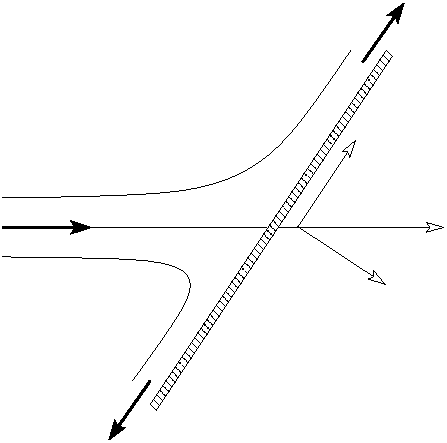
\includegraphics[width=6cm]{jet_impact.pdf}}
      \put(20, 40){$P_a$}
      \put(60, 40){$y$}
      \put(65, 20){$x$}
      \put(72, 30){$X$}
      \put(20, 40){$P_a$}
      \put(0, 27){$\vec{V}, \, q_m$}
      \put(50, 60){$\vec{V}', \, q_m'$}
      \put(10, 0){$\vec{V}'', \, q_m''$}
    \end{picture}
  \end{center}
  \mycaption{Jet plan impactant sur une plaque inclin\'ee.}
  \label{fig:jet_impact}
\end{figure}

Un jet d'eau bidimensionnel s'\'ecoulant \`a vitesse $\vec{V}$ (d\'ebit $q_m$) impacte 
une plaque plane inclin\'ee d'un angle $\alpha$ par rapport \`a
l'horizontale $X$ (fig.~\ref{fig:jet_impact}). 
On veut d\'eterminer la force exerc\'ee par le jet sur la plaque.
On note $q_m'$ et $q_m''$ les d\'ebits correspondant aux vitesses
$\vec{V}\,'$ et $\vec{V}\,''$ de l'\'ecoulement de part et d'autre
de l'impact.
On supposera les effets visqueux n\'egligeables, ainsi que l'effet de la pesanteur.
\begin{enumerate}
\item 
  Montrer que $V = V' = V''$.
\item 
  Exprimer la conservation du d\'ebit massique.
\item 
  D\'eterminer la force $\vec{F}$ exerc\'ee par les fluides sur la plaque.
  On exprimera les composantes $F_x$, $F_y$ et $F_X$.
\item 
  Calculer $q_m'$ et $q_m''$ en fonction de $q_m$ et $\alpha$.
\item 
  A quelles conditions les effets visqueux sont-ils effectivement n\'egligeables ?
\end{enumerate}




\subsection{Tube de pitot}


\begin{figure}[htb]
  \begin{center}
      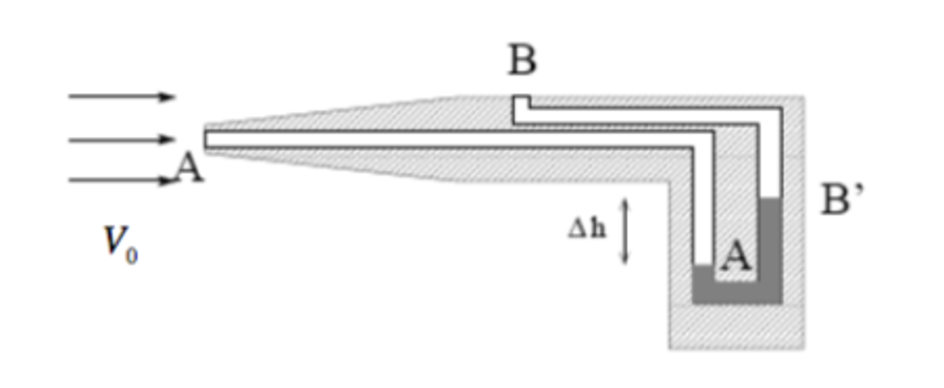
\includegraphics[width=.7\linewidth]{Pitot.pdf}
      \end{center}
      \vspace{-1cm}
\end{figure}

{\em Exercice complémentaire ; Correction disponible sur l'espace Moodle du cours de Mécanique des fluides de L2 (TD6, exercice 9)}.

Pour mesurer la vitesse $U_0$ de vehicules se déplaçant à grande vitesse dans l'air (masse volumique de l’air $\rho_a = 1.225kg/m^3$ ),  on utilise généralement des sondes de Pitot. Dans le manomètre en U du tube de Pitot, on utilise un liquide de masse volumique connue, de l'eau par exemple ($\rho_e = 1000kg.m^3$). On prendra $g = 9.81 m/s^2$.

La dénivellation indiquée dans le manomètre en U étant $h =10 cm$ , calculer la vitesse $U_0$.




%--------------------------------------------------------------------------------------------------
\subsection{Ventilation d'un tunnel (d'apr\`es examen 2008)}
%--------------------------------------------------------------------------------------------------

On consid\`ere un tunnel horizontal de section $S$ uniforme, ventil\'e par un soufflage d'air 
frais comme indiqu\'e sur la figure~\ref{fig:tunnel}. 
L'air souffl\'e \`a la vitesse $U_s$ dans un conduit de section $s$ se m\'elange \`a l'air 
du tunnel entre les sections 1 et 2. 
Dans la partie amont du tunnel (partie gauche), le soufflage peut induire un \'ecoulement 
vers la droite comme sur la figure, ou vers la gauche. On veut d\'eterminer les conditions 
r\'ealisant l'un ou l'autre \'ecoulement. 
Dans tout le probl\`eme, on n\'egligera les effets visqueux, et on consid\`erera l'\'ecoulement
isovolume, stationnaire, et uniforme dans toute section du tunnel, sauf entre les sections 1 et 2.

\begin{figure}[hbt]
  \begin{center}
    \setlength{\unitlength}{1mm}
    \begin{picture}(150, 40)(0, 5)
      \put(0, 0){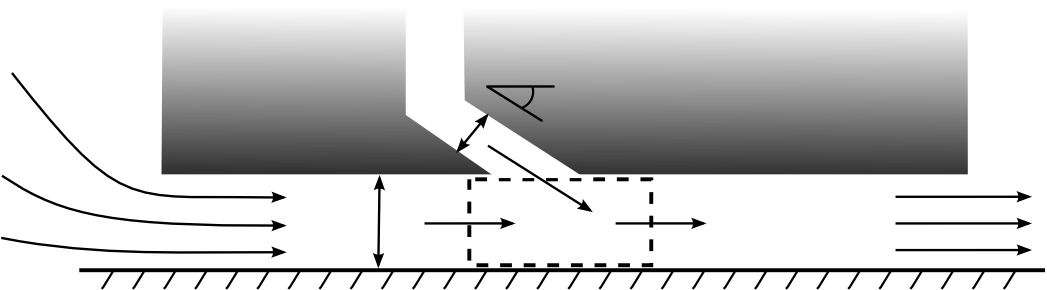
\includegraphics[width=15cm]{tunnel_ventile.png}}
      \put(0, 37){$p_a$} %, u = 0
      \put(145, 20){$p_a$}
      \put(65, 23){$s$}
      \put(50, 8){$S$}
      \put(78, 26){$\alpha$}
      \put(85, 12){$U_s$}
      \put(62, 11){$U_1$}
      \put(99, 11){$U_2$}
    \end{picture}
  \end{center}
  \mycaption{Sch\'ema du tunnel ventil\'e.}
  \label{fig:tunnel}
\end{figure}

\begin{enumerate}

\item 
  On consid\`ere que l'\'ecoulement correspond \`a la figure : 
  au voisinage de l'entr\'ee du tunnel, l'air atmosph\'erique est acc\'el\'er\'e progressivement, 
  alors qu'il sort du tunnel sous la forme d'un jet.
  \begin{enumerate}
  \item 
    Ecrire la relation de Bernoulli pour une ligne de courant entre l'ext\'erieur du tunnel 
    (infini amont) et la section 1.
  \item 
    Quelle est la pression de l'air \`a la sortie du tunnel~? 
    En d\'eduire, en utilisant la relation de Bernoulli, la pression dans la section 2.
  \item 
    Appliquer le bilan int\'egral de quantit\'e de mouvement pour 
    le volume de contr\^ole limit\'e par les parois du tunnel, les sections 1 et 2 et 
    la section de soufflage, d'aire $s/\sin \alpha$ o\`u $\alpha$ est l'angle du conduit 
    de soufflage avec l'axe du tunnel. 
    On consid\`erera l'angle $\alpha$ petit, soit $\cos \alpha \approx 1$.
  \item 
    Ecrire la relation liant $U_s$, $U_1$ et $U_2$, issue de la conservation de la masse.
  \item 
    D\'eduire des \'equations \'etablies ci-dessus la relation quadratique donnant 
    la vitesse normalis\'ee $u = U_1/U_s$ en fonction du rapport des sections $r = s/S$. 
  \item 
    Montrer qu'il n'existe de solution correspondant \`a la figure que si le rapport des 
    sections $r$ est inf\'erieur \`a une valeur critique que l'on pr\'ecisera.
  \item 
    Tracer l'\'evolution de $u$ en fonction de $r$, en pr\'ecisant les points remarquables 
    de la courbe. On donnera en particulier la valeur de $r$ qui maximise l'entra\^{\i}nement 
    d'air, et la valeur de ce maximum de $u$.
  \end{enumerate}
  
\item 
  Lorsque le rapport des sections exc\`ede la valeur critique d\'etermin\'ee ci-dessus, 
  l'\'ecoulement dans la partie amont du tunnel s'inverse. 
  Aux deux extr\'emit\'es du tunnel, l'air sort sous la forme d'un jet.
  \begin{enumerate}
  \item 
    En proc\'edant de fa\c{c}on similaire \`a la question pr\'ec\'edente, 
    d\'eterminer la vitesse normalis\'ee $u$ en fonction du rapport des sections $r$.
  \item 
    V\'erifier que la vitesse $u$, en tant que fonction de $r$, ne subit pas de discontinuit\'e 
    entre les deux r\'egimes d'\'ecoulement.
  \item 
    Pour un tunnel de 6 m\`etres de diam\`etre et des vitesses d'\'ecoulement de l'ordre 
    du m\`etre par seconde, le fait de n\'egliger les effets visqueux vous para\^{\i}t-il 
    justifi\'e ?
  \end{enumerate}
  
\end{enumerate}



\subsection{Estimation de la traînée d'un cylindre (Exam mai 2017)}


On étudie l'écoulement stationnaire autour d'un cylindre fixe de rayon $a$ et de longueur infinie dans la direction $z$ (écoulement bidimensionnel dans le plan $(x,y)$ ). 
Le fluide est considéré comme un liquide incompressible de masse volumique $\rho$ constante et de viscosité $\nu$. On néglige l'effet de la pesanteur.
On cherche a estimer la force 
${\bf F} = F_x {\bf e_x} + F_y {\bf e_y} $ exercée par le fluide sur le cylindre a partir de bilans intégraux.

%Loin du cylindre, l'écoulement est supposé uniforme, de direction $\myvec{e}_x$ et de valeur %$U_0$, et la pression est également uniforme et vaut $P_0$.


\begin{figure}[htb]
  \begin{center}
      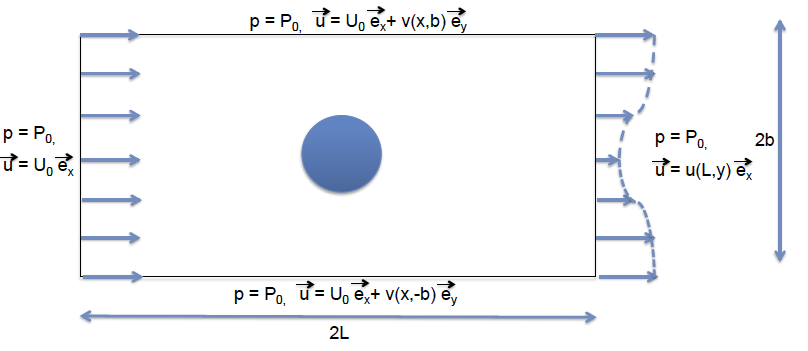
\includegraphics[width=.9\linewidth]{Cylindre_Bilan.png}
      \end{center}
      \vspace{-1cm}
\end{figure}

%La modélisation potentielle des deux parties précédentes ne permet pas de prédire la force de traînée, qui est due aux frottements visqueux à la surface du cylindre. Dans cette partie
%on cherche à estimer cette force de traînée par un bilan intégral dans le cas non tournant ($\Omega = 0$),  a partir de la loi de vitesse observée dans le sillage du cylindre à une distance $L$ de celui-ci.

%On cherche à estimer la force de traînée par un bilan intégral,  
%a partir de la loi de vitesse observée dans le sillage du cylindre à une distance $L$ de celui-ci.
 On considère pour cela un volume de contrôle correspondant à un domaine parallélépipédique 
 de largeur $2b$, longueur $2L$, et profondeur $2H$ (dans la direction z).  Les champ de vitesse ${\bf u} = u {\bf e_x} + v {\bf e_y} $  et de pression sur les frontières de ce volume de contrôle sont indiqués sur la figure. %Les lois $v(x,\pm b)$ et $u(L,y)$ sont 
 La troisième composante de vitesse $w$ est nulle sur toutes les frontières du domaine.
 On suppose que les effets visqueux sont négligeables loin du cylindre (y compris sur les frontières du volume de contrôle).

\begin{enumerate}

\item Ecrire un bilan de masse sur le volume de contrôle, et en déduire une relation intégrale reliant $U_0$, $u(L,y)$, $v(x,-b)$ et $v(x,b)$.
(ici et dans la question suivante on ne cherchera pas à calculer les intégrales apparaissant dans l'expression).


\item Ecrire un bilan de quantité de mouvement (théorème d'Euler) projeté dans la direction $x$, et en déduire une expression de la traînée (composante $F_x$ de la force exercée) sur le cylindre en fonction du champ de vitesse sur les frontières du domaine.


%\item Ecrire également un bilan de masse, et en déduire une relation intégrale reliant $u(L,y)$, 
%$v(x,-b)$ et $v(x,b)$.

\item En combinant les équations obtenues aux deux questions précédentes, montrez que la force de traînée peut être estimée par l'équation suivante :
$
F_x = 2 H \int_{-b}^{b} u(L,y) \left( U_0 - u(L,y) \right) dy 
$


\item
Application. On suppose qu'en sortie le profil de vitesse peut être approximé par la loi suivante: 
$$
u(L,y) = \left\{ \begin{array}{ll} U_0 \quad & |y|> a \\ 0.7 U_0 \quad & |y|< a \end{array}
\right.
$$

En déduire le coefficient de traînée $C_x = F_x / (\rho U_0^2 a H)$.


\item A partir d'un bilan de quantité de mouvement projeté dans la direction $y$, donnez une expression de la portance (composante $F_y$ de la force exercée) en fonction de la vitesse sur les frontières du domaine. A quelle condition cette portance est-elle nulle ? interprétez physiquement.


\end{enumerate}






\comment{
%--------------------------------------------------------------------------------------------------
\subsection{Attirer en soufflant \exonormal}
%--------------------------------------------------------------------------------------------------

On consid\`ere deux disques parall\`eles, de diam\`etre $D$, s\'epar\'es d'une distance $d \ll D$ (fig.~\ref{fig:interdisques}). De l'air, amen\'e par un tube normal aux disques avec une vitesse $V_c$, p\'en\`etre au centre du disque sup\'erieur par une ouverture de diam\`etre $d \ll D$. Au-del\`a de la section d'entr\'ee, l'air s'\'ecoule radialement  pour d\'eboucher dans l'atmosph\`ere. On n\'eglige les effets visqueux. 

\begin{figure}[htb]
\begin{center}
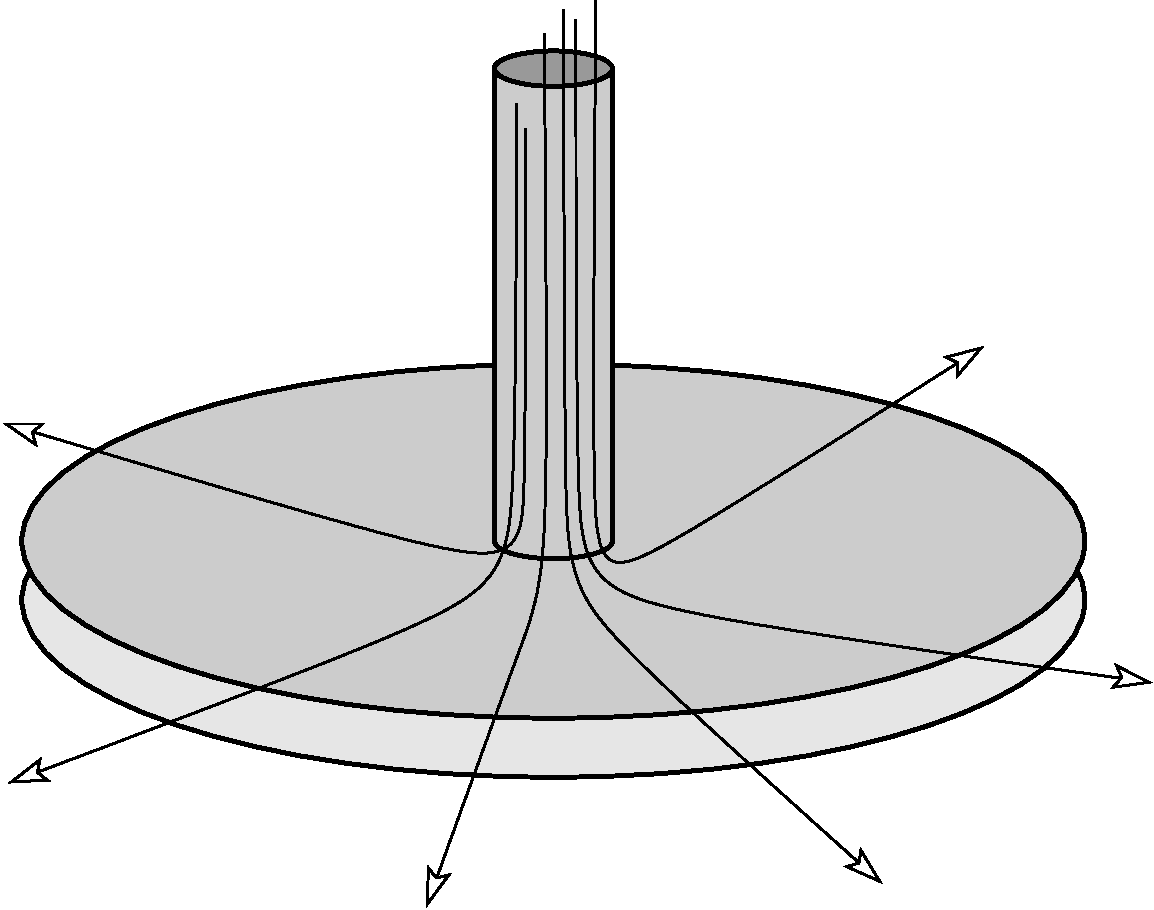
\includegraphics[width=8cm]{interdisques}
\end{center}
\mycaption{Ecoulement inter disques.}
\label{fig:interdisques}
\end{figure}

On notera $r$ la distance d'un point \`a l'axe $z$ des deux disques. Dans tout le probl\`eme, on admet que le module de la vitesse entre les deux disques ne d\'epend que de $r$ (sauf dans la zone $r<d/2$ o\`u les lignes de courant changent de direction). Dans la section de sortie $r=D/2$, la pression est \'egale \`a la pression atmosph\'erique $P_a$.

\begin{enumerate}
\item Calculer la vitesse $V(r)$ entre les deux disques pour $d/2<r<D/2$.
Comparer avec $V_c$.
\item Donner la valeur de la pression $P_c$ dans la conduite en fonction
de $V_c$ et $P_a$.
\item D\'eterminer la loi de pression $p(r)$ entre les deux disques pour $d/2<r<D/2$.
Comparer avec $P_a$.
\item Calculer la r\'esultante des forces subies par le disque sup\'erieur de la part
des fluides qui l'entourent pour $d/2<r<D/2$.
Y a-t'il r\'epulsion ou attraction~?
\item On surestime la pression aux points du disque inf\'erieur $r<d/2$ 
en la prenant \'egale \`a la pression en $0$.
Reprendre la question pr\'ec\'edente dans le cadre de cette hypoth\`ese.
\end{enumerate}


%--------------------------------------------------------------------------------------------------
\subsection{Lance d'incendie (d'apr\`es examen 2005) \exonormal}
%--------------------------------------------------------------------------------------------------

La lutte contre les incendies hors zone urbaine et particuli\`erement en
zone dite ``s\`eche'' b\'en\'eficie de l'aide d'appoint d'unit\'es mobiles
transportant un syst\`eme autonome constitu\'e d'un r\'eservoir d'eau,
d'une pompe et d'une lance \`a incendie embarqu\'es
sur un v\'ehicule tout terrain.
On s'int\'eresse dans ce probl\`eme \`a la description de certains aspects
du fonctionnement de ce syst\`eme.

L'eau est mise sous pression par un compresseur qui impose une pression
en entr\'ee de lance de $P_1 = P_0 + \varphi$ o\`u $P_0 = 10^5$ Pa 
d\'esigne la pression atmosph\'erique ambiante et $\varphi > 0$ la surpression,
de l'ordre de quelques bars.
La lance \`a incendie est reli\'ee au compresseur par un tuyau flexible,
et est maintenue par un support orientable.
Le diam\`etre d'entr\'ee de la lance est $D = 5$ cm, correspondant
\`a une section $S_1$.
La lance forme une conduite convergente, de section de sortie $S_0<S_1$. La surface lat\'erale de la lance est not\'ee $\Sigma$.

On rappelle que la masse volumique de l'eau est $\rho = 10^3 \, \mbox{kg/m}^3$
et sa viscosit\'e cin\'ematique $\nu = 10^{-6} \, \mbox{m}^2\mbox{/s}$.

\begin{figure}[htbp]
\begin{center}
\setlength{\unitlength}{1mm}
\begin{picture}(110, 30)
\put(0, 0){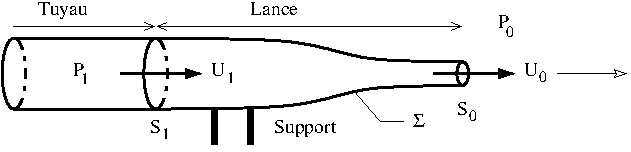
\includegraphics[width=10cm]{lance.pdf}}
\put(100, 10){$\vec{e}_x$}
\end{picture}
\end{center}
\mycaption{Mod\`ele de lance \`a incendie.}
\label{fig:lance}
\end{figure}

\begin{enumerate}
\item[]
\item
En supposant que l'ensemble reste globalement 
\`a un m\^eme niveau horizontal pendant le fonctionnement
de la lance, montrer que l'on peut n\'egliger l'influence de la pesanteur
dans cette configuration.
%\item[]
\item[]
Dans un premier temps, la lance d'incendie est ferm\'ee en $S_0$ :
il n'y a donc pas \'ecoulement.
\item
Calculer la r\'esultante $\vec{F}_0$ des forces de pression 
exerc\'ees sur la section
$S_0$ par l'eau sous pression dans la lance et l'air \`a pression
atmosph\'erique, en fonction de $\varphi$ et $S_0$.
\item
Calculer la r\'esultante $\vec{F}_1$ des forces de pression qui s'exercent
cette fois-ci sur la totalit\'e de la paroi de la lance
$S_0 \cup \Sigma$ en fonction de $\varphi$ et $S_1$.
\\
On pourra utiliser sans la red\'emontrer l'\'egalit\'e math\'ematique
suivante :
\[
\int\!\!\!\int_{\partial \Omega} \vec{n} \, \mbox{dS} = \vec{0}
\]
o\`u $\partial \Omega$ d\'esigne une surface \textit{ferm\'ee} de normale
sortante $\vec{n}$.
\item
En d\'eduire la force $\vec{R}$ 
exerc\'ee par l'ensemble \{tuyau et support\} sur la lance.
\item[]
%\item[]
On ouvre maintenant la lance en $S_0$ : un jet d'eau sort \`a vitesse $U_0$
dans l'air \`a pression atmosph\'erique $P_0$.
\item
Calculer la vitesse $U_1$ en entr\'ee de la lance et
la vitesse $U_0$ en sortie, en fonction de $\varphi$, $\rho$ et du rapport
des section $\alpha = S_1/S_0 > 1$ (on admettra que la vitesse est uniforme dans toute section).
\item
Donner alors l'expression du nombre de Reynolds $Re$ en entr\'ee de la lance
d'incendie en fonction en particulier de $\varphi$. \\
Application num\'erique : calculer son ordre de grandeur pour un rapport
de section $\alpha=2$ et un r\'egime de fonctionnement correspondant \`a
$\varphi = 2P_0$.
En d\'eduire la nature laminaire ou turbulente du r\'egime d'\'ecoulement
dans la lance. L'hypoth\`ese de vitesse uniforme faite \`a la quesion pr\'ec\'edente est-elle justifi\'ee ?
\item
Donner l'expression du d\'ebit massique $\dot{m}$ puis du d\'ebit volumique $q$
et calculer leur valeur dans le r\'egime de fonctionnement d\'ecrit dans
la question pr\'ec\'edente.
\item
Donner l'expression de la r\'esultante $\vec{F}$
des forces de pression exerc\'ees par les fluides (eau et air)
sur la paroi $\Sigma$ de la lance, en fonction de $q$, $\rho$, $\alpha$
et $S_1$.
Dans quel sens s'exerce cette force~?
\item
Comparer cette force avec la force $\vec{R}$ exerc\'ee par le tuyau
et le support dans le cas sans \'ecoulement (on pourra pour ce faire
\'ecrire cette derni\`ere force en fonction de $q$, $\rho$, $\alpha$
et $S_1$).
Que pourrait-on en d\'eduire sur le mouvement de la lance au moment
de la mise en \'ecoulement \`a l'ouverture de $S_0$~?
\item
En consid\'erant un bilan int\'egral de quantit\'e de mouvement pour l'ensemble
du syst\`eme embarqu\'e, quelle est la force induite par le jet d'eau sur
le v\'ehicule d'intervention~? 
\end{enumerate}
}


\comment{

%%%%%%%%%%%%%%%%%%%%%%%%%%%%%%%%%%%%%%%%%%%%%%%%%%%%%%%%%%%%%%%%%%%%%%%%%%%%%%%
\subsection{Siphon}
%%%%%%%%%%%%%%%%%%%%%%%%%%%%%%%%%%%%%%%%%%%%%%%%%%%%%%%%%%%%%%%%%%%%%%%%%%%%%%%

\noindent
\begin{tabular}{lp{1cm}r}
\begin{minipage}{7cm}
Un siphon permet l'\'ecoulement de l'eau d'un r\'eservoir
de grandes dimensions.
Il est constitu\'e d'un tuyau de diam\`etre constant qui s'\'el\`eve
\`a une hauteur $H$ au-dessus du niveau de la surface libre.

Calculer la valeur du d\'ebit maximum que l'on peut obtenir avec ce dispositif
sans qu'il se produise de cavitation (pression quasi nulle en un point
du siphon~: dans ce cas l'eau devient gazeuse et les bulles de gaz ainsi
g\'en\'er\'ees, plus l\'eg\`eres que le liquide, viennent se loger
en haut du siphon, provoquant un risque de d\'esamor\c{c}age).
Quelle est alors l'altitude de la sortie du siphon ?
\end{minipage}
& &
\begin{minipage}{7cm}
\begin{center}
%\input{Figures_FluidesL2/siphon.pstex_t}
\end{center}
\end{minipage}
\end{tabular}


%%%%%%%%%%%%%%%%%%%%%%%%%%%%%%%%%%%%%%%%%%%%%%%%%%%%%%%%%%%%%%%%%%%%%%%%%%%%%%%
\subsection{D\'ebit d'un barrage}
%%%%%%%%%%%%%%%%%%%%%%%%%%%%%%%%%%%%%%%%%%%%%%%%%%%%%%%%%%%%%%%%%%%%%%%%%%%%%%%

Une vanne retient partiellement l'eau d'un barrage de grandes dimensions
dans lequel la hauteur d'eau, fix\'ee, est $H$.
Calculer la hauteur $h$ de sortie correspondant au d\'ebit maximum.

\begin{figure}[hbt]
\begin{center}
%\input{Figures_FluidesL2/barrage.pstex_t} \hskip 2cm \input{../FIGURES/clepsydre.pstex_t}
\end{center}
\caption{(a) Barrage. (b) Clepsydre.} 
\label{fig:baclep}
\end{figure}

%%%%%%%%%%%%%%%%%%%%%%%%%%%%%%%%%%%%%%%%%%%%%%%%%%%%%%%%%%%%%%%%%%%%%%%%%%%%%%%
\subsection{Clepsydre}
%%%%%%%%%%%%%%%%%%%%%%%%%%%%%%%%%%%%%%%%%%%%%%%%%%%%%%%%%%%%%%%%%%%%%%%%%%%%%%%

La clepsydre est une horloge \`a eau connue aussi bien des Egyptiens que des
Am\'erindiens ou des Grecs.
Si le cadran solaire donne l'heure pendant le jour, 
la clepsydre fait la m\^eme chose la nuit, et elle mesure en plus
des dur\'ees plus br\`eves avec une bonne pr\'ecision. 
Un vase perc\'e d'un trou (section $S_0$) laisse couler de l'eau.
Des graduations situ\'ees \`a l'int\'erieur permettent de mesurer des
intervalles de temps.
On souhaite d\'eterminer la forme du vase
telle que la surface libre du liquide, d'aire $S(z)$, s'abaisse 
proportionnellement au temps.
\begin{enumerate}
\item
Calculer la vitesse d'\'ejection de l'eau en sortie ($z=0$).
\item
Donner la loi de variation de l'aire $S(z)$ de la clepsydre.
\item
Dans le cas o\`u le r\'eservoir est de section circulaire,
en d\'eduire la loi de variation de $R(z)$.
\end{enumerate}

%\newpage

%\setlength{\oddsidemargin}{-1cm}
%\setlength{\evensidemargin}{-1cm}


%%%%%%%%%%%%%%%%%%%%%%%%%%%%%%%%%%%%%%%%%%%%%%%%%%%%%%%%%%%%%%%%%%%%%%%%%%%%%%%
\subsection{Ecoulements \`a surface libre}
%%%%%%%%%%%%%%%%%%%%%%%%%%%%%%%%%%%%%%%%%%%%%%%%%%%%%%%%%%%%%%%%%%%%%%%%%%%%%%%

\begin{enumerate}
\item
Une nappe d'eau s'\'ecoule sur un sol qui pr\'esente une d\'enivellation $H>0$
(bosse).
En d\'esignant par $h_1$ et $V_1$ la hauteur d'eau et la vitesse \`a l'infini
amont, montrer que $h_2 > h_1$ correspond \`a $V_1>\sqrt{gh_1}$
(r\'egime torrentiel), et r\'eciproquement
$h_2 < h_1$ si $V_1<\sqrt{gh_1}$ (r\'egime fluvial),
o\`u $h_2$ est la hauteur d'eau \`a l'aplomb de la d\'enivellation.
On notera $V_2$ la vitesse de l'\'ecoulement juste au-dessus de la
d\'enivellation, et on supposera que l'\'ecoulement est uniforme dans chaque
section.
\item
Reprendre l'exercice pr\'ec\'edent et retrouver les deux r\'egimes
d'\'ecoulement en laissant le fond horizontal, mais en imposant une diminution
de la section $e$ de passage par un r\'etr\'ecissement du canal
(\'ecoulement entre les piles d'un pont par exemple).
\end{enumerate}

\begin{figure}[hbt]
\begin{center}
%\input{Figures_FluidesL2/torrent.pstex_t} \hskip 2cm \input{Figures_FluidesL2/pont.pstex_t}
\end{center}
\caption{Ecoulements \`a surface libre.}
\label{fig:esl}
\end{figure}

%%%%%%%%%%%%%%%%%%%%%%%%%%%%%%%%%%%%%%%%%%%%%%%%%%%%%%%%%%%%%%%%%%%

\newpage
\subsection{Le diffuseur de parfum }


%\documentclass[12pt,a4]{article}
\usepackage[french]{babel}
\usepackage[T1]{fontenc} 

\usepackage{floatflt,fancyheadings,amssymb,color}
\usepackage{psfig,epsfig}
\usepackage{pictex}
\usepackage{charter}
\hoffset=-4cm 
\voffset=-4cm
\topmargin=15mm
\headheight=5mm
\headsep=15mm
\textheight=260mm
\oddsidemargin=30mm
\evensidemargin=30mm
\textwidth=170mm
\pagestyle{plain}
\renewcommand{\textfraction}{.10}
\newcommand{\derp}[2]{ \frac{ \partial #1 }{ \partial #2}}
\newcommand{\dsp} {\displaystyle}
\newcommand{\torseur}[4]{
\Biggl\{ {\cal #1} (#2)\Biggr \} = 
\left \{ \begin{array}{c}
#3  \\
#4 
\end{array} \right\} 
}
    
    

\begin{document}
\sf 


\begin{center}
  Licence II math�matiques \& M�canique, Universit\'e Paul Sabatier.
 \vspace{0.6cm}
 
Th�me 4 (suite)

 {\bf \Large Le diffuseur de parfum }


\documentclass[12pt,a4]{article}
\usepackage[french]{babel}
\usepackage[T1]{fontenc} 

\usepackage{floatflt,fancyheadings,amssymb,color}
\usepackage{psfig,epsfig}
\usepackage{pictex}
\usepackage{charter}
\hoffset=-4cm 
\voffset=-4cm
\topmargin=15mm
\headheight=5mm
\headsep=15mm
\textheight=260mm
\oddsidemargin=30mm
\evensidemargin=30mm
\textwidth=170mm
\pagestyle{plain}
\renewcommand{\textfraction}{.10}
\newcommand{\derp}[2]{ \frac{ \partial #1 }{ \partial #2}}
\newcommand{\dsp} {\displaystyle}
\newcommand{\torseur}[4]{
\Biggl\{ {\cal #1} (#2)\Biggr \} = 
\left \{ \begin{array}{c}
#3  \\
#4 
\end{array} \right\} 
}
    
    

\begin{document}
\sf 


\begin{center}
  Licence II math�matiques \& M�canique, Universit\'e Paul Sabatier.
 \vspace{0.6cm}
 
Th�me 4 (suite)

 {\bf \Large Le diffuseur de parfum }


\input{parfum.pstex_t}

\end{center}


Le dispositif repr�sent� sur la figure est utilis� pour diffuser du parfum.
Un courrant d'air, de d�bit volumique $q$ constant, circule dans un conduit
pr�sentant un r�tr�cissement. Un tuyau, raccord� au r�cipient contenant le 
parfum, est dispos� au col. Si le d�bit d'air est suffisant, le parfum
est aspir� dans le tuyau, et circule avec un d�bit volumique $q_l$.
On suppose le d�bit volumique du parfum faible devant celui de l'air,
de sorte que le d�bit volumique en sortie est $q+q_l \approx q$.

On note $\rho_a$ et $\rho_l$ les masses volumiques de l'air et du liquide,
$S$ et $S_c$ les sections en entr�e et au col, et $\Delta h$ la hauteur entre
la surface du liquide dans le r�cipient et la sortie du tuyau.

1/ Montrez qu'un d�bit d'air minimal est n�cessaire pour que le parfum
soit diffus�.
Lorsque le d�bit d'air est inf�rieur � cette valeur, donnez la hauteur atteinte
dans le tube par le parfum.

2/ Lorsque le d�bit d'air est sup�rieur � la valeur critique, calculez
le d�bit volumique de parfum diffus�.

3/ Repr�sentez la fraction volumique de parfum, $q_l/q$, en fonction de $q$.



Remarque : Un dispositif du m�me type est utilis� dans certains carburateurs
(mais ca sent moins bon).

\end{document}


\end{center}


Le dispositif repr�sent� sur la figure est utilis� pour diffuser du parfum.
Un courrant d'air, de d�bit volumique $q$ constant, circule dans un conduit
pr�sentant un r�tr�cissement. Un tuyau, raccord� au r�cipient contenant le 
parfum, est dispos� au col. Si le d�bit d'air est suffisant, le parfum
est aspir� dans le tuyau, et circule avec un d�bit volumique $q_l$.
On suppose le d�bit volumique du parfum faible devant celui de l'air,
de sorte que le d�bit volumique en sortie est $q+q_l \approx q$.

On note $\rho_a$ et $\rho_l$ les masses volumiques de l'air et du liquide,
$S$ et $S_c$ les sections en entr�e et au col, et $\Delta h$ la hauteur entre
la surface du liquide dans le r�cipient et la sortie du tuyau.

1/ Montrez qu'un d�bit d'air minimal est n�cessaire pour que le parfum
soit diffus�.
Lorsque le d�bit d'air est inf�rieur � cette valeur, donnez la hauteur atteinte
dans le tube par le parfum.

2/ Lorsque le d�bit d'air est sup�rieur � la valeur critique, calculez
le d�bit volumique de parfum diffus�.

3/ Repr�sentez la fraction volumique de parfum, $q_l/q$, en fonction de $q$.



Remarque : Un dispositif du m�me type est utilis� dans certains carburateurs
(mais ca sent moins bon).

\end{document}



Le dispositif représenté sur la figure est utilisé pour diffuser du parfum.
Un courrant d'air, de débit volumique $q$ constant, circule dans un conduit
présentant un rétrécissement. Un tuyau, raccordé au récipient contenant le 
parfum, est disposé au col. Si le débit d'air est suffisant, le parfum
est aspiré dans le tuyau, et circule avec un débit volumique $q_l$.
On suppose le débit volumique du parfum faible devant celui de l'air,
de sorte que le débit volumique en sortie est $q+q_l \approx q$.

On note $\rho_a$ et $\rho_l$ les masses volumiques de l'air et du liquide,
$S$ et $S_c$ les sections en entrée et au col, et $\Delta h$ la hauteur entre
la surface du liquide dans le récipient et la sortie du tuyau.

1/ Montrez qu'un débit d'air minimal est nécessaire pour que le parfum
soit diffusé.
Lorsque le débit d'air est inférieur à cette valeur, donnez la hauteur atteinte
dans le tube par le parfum.

2/ Lorsque le débit d'air est supérieur à la valeur critique, calculez
le débit volumique de parfum diffusé.

3/ Représentez la fraction volumique de parfum, $q_l/q$, en fonction de $q$.



Remarque : Un dispositif du même type est utilisé dans certains carburateurs
(mais ca sent moins bon).

}

% !TEX root = TD_fluides_part2.tex


\setcounter{section}{7}

\section{Ecoulements Inertiels II : Ecoulements potentiels}

\setcounter{subsection}{-1}


\subsection{Ecoulement autour d'un cylindre : effet Magnus} 

{\em Correction détaillée sur moodle.}


\vspace{1cm}

On étudie l'écoulement bidimensionnel d'un fluide incompressible de masse volumique uniforme 
$\rho$, défini par le potentiel des vitesses suivant, 
exprimé en coordonnées polaires $(r,\theta)$. :  


  \begin{equation}
   \Phi(r,\theta) =  U_0   \cos \theta \left( r + \frac{a^2}{r}\right)  
   + \frac{\Gamma \theta }{2 \pi}
  \end{equation}
  
Dans cet exercice on néglige la gravité.


\begin{enumerate}
\item Rappelez la définition et les conditions d'existence d'un écoulement potentiel.

\item Exprimez les composantes $u_r, u_\theta$ du champ de vitesse. Vérifiez que l'écoulement est bien à divergence nulle.

\item 
Que deviennent ces expressions sur le cercle de rayon $a$ et à l'infini 
($r \rightarrow \infty$) ? 

Conclure que cet écoulement est solution des équations d'Euler stationnaire
et représente l'écoulement autour d'un cylindre de rayon $a$.

\item Montrez que cet écoulement admet également une fonction de courant définie par
$$
\psi(r,\theta) = U_0   \sin \theta \left( r - \frac{a^2}{r}\right)  
   - \frac{\Gamma}{2 \pi} \ln r/.
 $$
Justifiez que les lignes de courant et les lignes isopotentielles forment des réseaux de courbes orthogonales.

%\item le programme  Matlab \verb|Ecoulement_Potentiel_cylindre.m| 

\item Discutez, suivant la valeur de $\Gamma$, le nombre et la position
des points d'arrêt sur la surface du cylindre (on suppose $\Gamma \leq 0$).

Représentez schématiquement la forme des lignes de courant pour 
différentes valeurs de $\Gamma$.


\item Exprimez le champ de pression $p(r,\theta)$ correspondant à cet écoulement.

Représentez graphiquement la loi de pression pariétale $p(r=a,\theta)$ en fonction de $\theta$,
pour plusieurs valeurs de $\Gamma$.


\item Calculez la force $\vec F$ (par unité de longueur),
exercée par le fluide sur le cylindre. 
Montrez que les composantes $F_x$ et $F_y$ de cette force
 v\'erifient $F_x = 0$ et $F_y = - \rho \Gamma
  U_0$. 
 
 \item Retrouvez ce résultat a partir d'un bilan de quantité de mouvement sur un volume de contrôle judicieusement choisi.
 
   
\item On suppose que le cylindre tourne selon son axe, à la vitesse angulaire
$\Omega$ (c'est à dire que son vecteur rotation est 
$\vec \Omega = \Omega \vec e_z$). 
Donnez, en coordonnées axisymétriques, la  vitesse d'un point situé 
sur la paroi du cylindre. Expliquez pourquoi l'approximation de fluide
parfait ne permet pas de calculer $\Gamma$ en fonction de $\Omega$.


\item L'étude des effets visqueux à l'intérieur de la couche limite {\em (Moore, 1953, Journal of Fluid Mechanics)} permet de montrer que si le cylindre tourne très vite $(\Omega \gg U_0/a)$,  
la circulation est reliée au taux de rotation par $\Gamma = 2 \pi a^2 \Omega$.
Donnez une interprétation physique de cette condition.

\item Montrer que dans ce cas 
$\overrightarrow{F} = 2 \pi \rho a^2 \overrightarrow{U}_0 \wedge \overrightarrow{\Omega}$
(formule de Magnus).

\end{enumerate}


%\subsection{Exercice complémentaire ??? } 

%L'ancien numéro 8, transvasement entre deux réservoirs, est un peu hors sujet...

%Si temps le permet, rajouter l'exercice oscillations dans un tube en U...



\subsection{Oscillations d'un pendule plongé dans un liquide}

Un pendule de masse $M$ attaché à une corde de longueur $L$ est un exemple bien connu d'oscilateur harmonique. Si les interactions avec le fluide sont négligées (ou si le pendule oscille dans le vide) on montre classiquement que la fréquence d'oscillation est donnée par 
$T = 2\pi/\omega_0$ avec $\omega_0 = \sqrt{g/L}$.

Dans le cas où le pendule oscille dans un liquide de masse volumique $\rho$, on observe que la fréquence est modifiée et donnée par la loi suivante :
\begin{equation}
\omega_0^2 = \frac{g (M - \rho V)}{L (M+\rho V C)}
\label{eq:omega0}
\end{equation}

où $V$ est le volume du pendule et $C$ un coefficient appelé "coefficient de masse ajoutée" 
qui dépend de sa forme (et vaut $C=1/2$ pour une sphère et $C=1$ pour un cylindre).



%Dans le cas ou l'oscillateur est un pendule (cylindre de rayon $a$ attaché à une corde de longueur $L$), oscillant dans un liquide, On observe également des différences notables par rapport au cas classique du pendule dans le vide pour lequel 

L'explication de cette modification de la fréquence, ainsi que la prédiction du temps d'amortissement du pendule, on suscité des débats dans la communauté scientifique au milieu du 19ème siècle. C'est Stokes (encore lui...) qui a finalement résolu le problème en 1850. Dans ce problème on va présenter une approche simplifiée de ce travail.


\begin{enumerate}

\subsubsection*{A. Questions préliminaires}


\item
On suppose que l'écoulement peut être modélisé en deux parties : un écoulement extérieur potentiel et une couche limite dominée par les effets visqueux et d'épaisseur $\delta$. 

Rappelez les hypothèses (a verifier a posteriori) permettant de justifier cette approximation.


\item Justifiez que la force exercée par l'écoulement sur la sphère est composée de 3 termes : 
$(i)$ la résultante de pression (motrice) 
$\myvec{F}_p = \iint - \hat{p} \myvec{n} dS$ qui peut être déterminée en fonction de l'écoulement potentiel et non pesant, $(ii)$ la poussée d'Archimède $-\rho V \myvec{g}$, et $(iii)$ l'effet du frottement visqueux $\myvec{F}_v$ dans les couches limites $F_v$.


\subsubsection*{B. Ecoulement potentiel autour d'une sphère en translation}
%On rappelle l'expression des opérateurs gradient et Laplacien en coordonnées sphériques.

La sphère se déplace à vitesse $\myvec{U} =U(t) \myvec{e_x}$ dans une direction $e_x$ supposée fixe.


On note $\myvec u = \gradient \Phi$ le champ de vitesse de l'écoulement {\em dans le repère relatif en mouvement avec la sphère}.

On introduit des coordonnées cartésiennes $x,y,z$ et des coordonnées sphériques 
$r,\theta,\varphi$.



On rappelle les expressions en coordonnées sphériques des opérateurs gradient et Laplacien :

$$
\gradient \Phi = \ddp{\Phi}{r} \myvec{e}_r 
+ \frac{1}{r}\ddp{\Phi}{\theta} \myvec{e}_\theta 
+ \frac{1}{r \sin \theta}\ddp{\Phi}{\varphi} \myvec{e}_\varphi
$$

$$
\Delta \Phi = \frac{1}{r^2} \ddp{}{r} \left( r^2 \ddp{\Phi}{r} \right) 
+ \frac{1}{r^2\sin \theta} \ddp{}{\theta} \left( \sin \theta \ddp{\Phi}{\theta} \right)
+ \frac{1}{r^2\sin^2 \theta} \ddp{^2\Phi}{\varphi^2} 
$$


%\begin{enumerate}
\item Donnez l'équation vérifiée par le potentiel ainsi que les conditions limites vérifiées par ce dernier sur la surface de la sphère ($r=a$) et loin de la sphère ($r \rightarrow \infty$).

\item On cherche une solution à variables séparées sous la forme :
$$
{\color{red} \Phi} (r,\theta) =  f(r) \cos \theta
$$
Donnez l'équation différentielle vérifiée par $f(r)$. 

\item En cherchant des solutions à cette équation sous forme de puissances de $r$, 
montrez que la solution est de la forme $f(r) = A r + B r^{-2}$ où $A$ et $B$ sont des constantes à déterminer.

\item A partir des conditions limites vérifiées en $r=a$ et $r= \infty$ déterminez les constantes $A$ et $B$.

\item En déduire que le champ de vitesse est donné par :

$$
u_r(r,\theta)= -U(t) \left( 1 - \frac{a^3}{r^3} \right) \cos \theta
$$ 
$$
u_\theta(r,\theta)
 = U(t) \left( 1 + \frac{a^3}{2r^3} \right) \sin \theta
 $$

Représentez schématiquement la structure de l'écoulement.

\subsubsection*{C. Champ de pression et force exercée sur la sphère due à l'écoulement potentiel}

Dans cette partie on ne tient pas compte de la gravité et du frottement visqueux, on s'intéresse uniquement à la force exercée par la sphère associée à l'écoulement potentiel.

%\item Justifiez que la force exercée par la sphère se décompose en 3 termes :
%$(i)$ une force hydrodynamique que l'on peut calculer a partir de 

\item A partir des équations d'Euler dans le repère relatif en mouvement avec la sphère ({\em non galliléen)}, démontrer une forme généralisée du second théorème de Bernouilli.

\item En déduire l'expression de la pression $p(a,\theta)$ exercée sur la surface du cylindre. 

\item Montrez que la force exercée sur l'objet par l'écoulement vaut :
$$
\myvec{F}_p = - \rho V C  \frac{ dU}{dt} \myvec{e}_x  , \quad \mbox{ avec } V = \frac{4 \pi a^3}{3} \mbox{ et } 
C = \frac{1}{2}
$$
%$$
%F_y = 0
%$$
%Quelle est l'interprétation physique des deux termes apparaissant dans $F_x$ ?

\item Que vaut la force si la sphère se déplace à vitesse uniforme ? Commentez ce résultat.

\item Que vaut la force si la sphère se déplace de manière uniformément accélérée ? Interprétez physiquement le résultat et donnez une interprétation géométrique au coefficient $C$.


\subsubsection*{D. Application : oscillations d'un pendule}

On considère maintenant le cas d'un pendule constitué d'une sphère de rayon $a$ et masse $m$ attaché à une ficelle de longueur $L$. 

On note $\phi(t)$ l'angle d'inclinaison du pendule, et on introduit un repère 
$(\myvec{e}_x, \myvec{e}_y, \myvec{e}_z)$ tel que la vitesse instantanée soit alignée avec l'axe $x$, c.a.d. : $\myvec{U} = U(t) \myvec{e}_x = L d \phi / dt$.

On admettra qu'on peut négliger les termes d'accélération centrifuge et de Coriolis, et que l'écoulement autour de la sphère et la force associé sont les mêmes que ce qu'on a calculé dans les questions précédentes.




\item En appliquant le principe fondamental de la dynamique à la sphère, projeté selon l'axe 
$\myvec{e_x}$, montrez que le mouvement est gouverné par l'équation différentielle suivante :

$$
(m+\rho VC) L
\frac{d^2 \phi}{d t^2} =  \myvec{F}_v \cdot \myvec{e_x} { \color{red} - }  (m-\rho V) g \phi
$$



\item Si les forces visqueuses sont négligeables, en déduire que le pendule oscille avec la période $T = 2\pi / \omega_0$ où $\omega_0$ est donné plus haut par l'équation (\ref{eq:omega0}).

\item 
Application numérique : calculez la période pour un pendule de dimensions $L=10cm$, $a=1cm$, dans les cas suivants :

$(i)$ Pendule en acier ($\rho_p = 7850$) dans l'eau ($\rho = 1000$)

$(ii)$ Pendule en PVC ($\rho_p = 1400$) dans l'eau ($\rho = 1000$)

$(ii)$ Pendule en verre ($\rho_p = 2500$) dans l'air ($\rho = 1.225$)

\subsubsection*{E. Estimation des effets visqueux}

\item Estimez l'épaisseur de la couche limite $\delta$ dans les 3 cas précédents. L'hypothèse de couche limite est-elle effectivement justifiée a posteriori ?

\item Dans le cas d'une sphère oscillant à la pulsation $\omega_0$, le calcul des forces de frottement dans les couches limites (du à Stokes) conduit à :

$$
\myvec{F}_v = - \frac{9}{4} \frac{V}{a}  \mu \frac{U(t)}{\sqrt{\frac{\nu}{\omega_0}}} \myvec{e}_x
$$   

Justifiez la forme de cette expression (on ne demande pas de démontrer le facteur 9/4 !).

\item
En supposant que l'effet des frottements visqueux est une petite correction par rapport au calcul précédent, montrez que l'on aboutit à une équation d'oscillateur harmonique amorti de la forme :

$$
\frac{d^2 \phi}{d t^2} + \frac{1}{\tau} \frac{d \phi}{d t} + \omega_0^2 \phi =0
$$

\item Donnez la valeur du temps d'amortissement $\tau$ du pendule pour les cas $(i)$, $(ii)$ et $(iii)$ définis plus haut.

\end{enumerate}


\comment{

%--------------------------------------------------------------------------------------------------
\subsection{Ascension d'une bulle parachute (d'après Davies \& Taylor, 1950) $^*$}
%--------------------------------------------------------------------------------------------------

\begin{figure}[hbt]
  \begin{center}
    \setlength{\unitlength}{1mm}
    \begin{picture}(100, 110)(0, 5)
      \put(0, 61){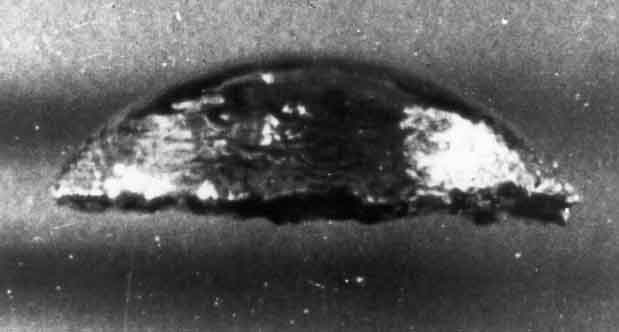
\includegraphics[width=7cm]{bubble_cap1}}
      \put(0, 0){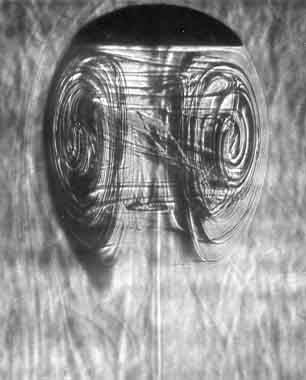
\includegraphics[height=4cm]{bubble_cap2}}
      \put(50, 0){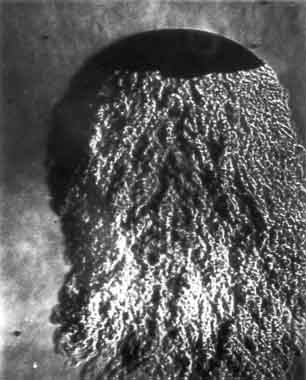
\includegraphics[height=4cm]{bubble_cap3}}
      \put(2, 109){\bf (a)}
      \put(2, 3){\bf (b)}
      \put(52, 3){\bf (c)}
    \end{picture}
  \end{center}
  \mycaption{(a) Photographie d'une bulle parachute en ascension
    (Davenport \textit{et al.}, 1967).
    Bulle avec sillage laminaire \`a $Re=180$ (b) et turbulent \`a $Re = 17000$ (c).
    D'après Wegener \& Parlange (1973).}
  \label{fig:cap_bubbles}
\end{figure}


\begin{figure}
  \begin{center}
%   \setlength{\unitlength}{1mm}
%    \begin{picture}(60, 65)(0, 5)
%      \put(0, 0){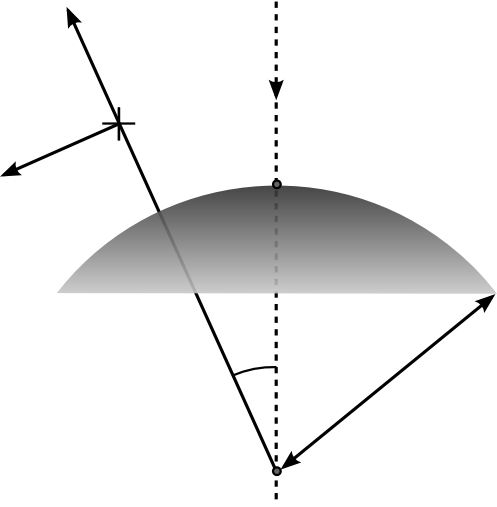
\includegraphics[width=6cm]{geometrie_bulle.png}}
%      \put(29, 3){$O$}
%      \put(2, 44){$\vec{e}_\theta$}
%      \put(12, 58){$\vec{e}_r$}
%      \put(30, 18){$\theta$}
%      \put(24, 21){\colorbox{white}{$r$}}
%      \put(29.5, 40){$S$}
%      \put(44.5, 14){\colorbox{white}{$R$}}
%      \put(16, 48){$M$}
%    \end{picture}
\vspace{-9cm}
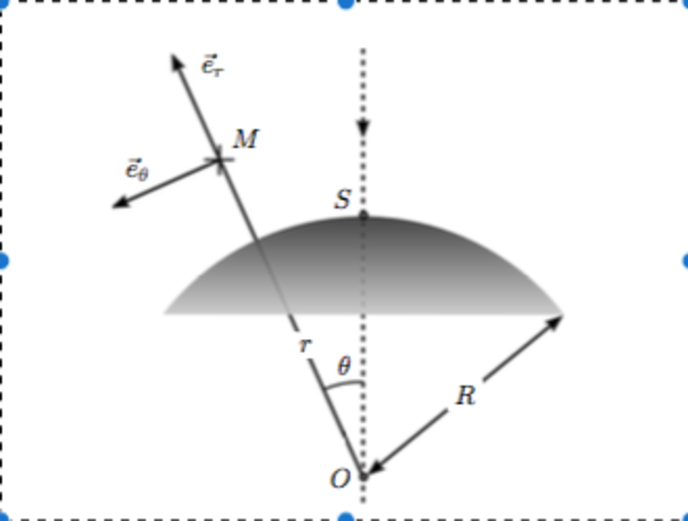
\includegraphics[width=15cm]{BulleTaylorShema.pdf}
\vspace{-8cm}
  \end{center}
  \mycaption{Param\`etres g\'eom\'etriques de l'\'ecoulement autour d'une bulle.}
  \label{fig:geometrie_bulle}
\end{figure}


L'exp\'erience montre que les bulles de gaz de quelques centim\`etres de diam\`etre qui remontent 
dans un liquide ont une forme de parachute (fig.~\ref{fig:cap_bubbles})~:
la partie avant de la bulle est sph\'erique et sa partie arri\`ere
est \`a peu pr\`es plate (calotte sph\'erique).
G. I. Taylor a \'etudi\'e exp\'erimentalement la relation entre la vitesse
d'ascension des bulles et le rayon de courbure de la partie avant.
Dans ses exp\'eriences, des bulles d'air s'\'el\`event dans du nitrobenz\`ene
(de viscosit\'e cin\'ematique $\nu = 0.015$ cm$^2$/s et de masse volumique
$\rho = 1.2$ g/cm$^3$).
Les rayons de courbures observ\'es sont compris entre $2.4$ et $4.8$ cm,
les vitesses d'ascension correspondantes entre $29$ et $48$ cm/s
et les dimensions transverses $2R\sin\theta_m$ entre $2.8$ et $6.2$ cm.

\begin{enumerate}

\item 
Dans les exp\'eriences d\'ecrites ci-dessus, quel est l'ordre de grandeur du nombre de Reynolds 
pour l'\'ecoulement de liquide ?
Conclusions.

\item Evaluez le nombre de Bond. En déduire que la pression le long de la surface de la bulle peut être considérée comme constante.


\item A partir du théorème de Bernouilli, donner une relation entre l'altitude 
$z= R \cos \theta$  et la vitesse $|\vec{u}(R,\theta)|$ sur la surface de la bulle.


%Evaluer la vitesse tangentielle du liquide au voisinage du point d'arr\^et $S$. 
%On pourra supposer que la pression \`a l'int\'erieur de la bulle est constante.

\item 
Taylor fait la remarque que l'\'ecoulement du liquide autour du sommet
de la calotte sph\'erique est peu diff\'erent de l'\'ecoulement potentiel
autour d'une sph\`ere donn\'e par
$$
u_r(r, \theta) = -U\left ( 1 - \frac{R^3}{r^3} \right ) \cos\theta
\quad \mbox{et} \quad
u_\theta(r, \theta) = U\left ( 1 + \frac{R^3}{2r^3} \right ) \sin \theta
$$
dans le r\'ef\'erentiel o\`u la bulle est immobile et o\`u le liquide
se d\'eplace \`a la vitesse $U$ loin de la bulle. 

%
%En comparant ces expressions avec les r\'esultats obtenus pr\'ec\'edemment, 
%d\'eterminer la vitesse d'ascension de la bulle. 


En déduire que la vitesse de la bulle est donnée par :
$$
U = \frac{2}{3} \sqrt{gR}
$$

\item
Confronter cette pr\'ediction th\'eorique aux valeurs obtenues exp\'erimentalement.

\end{enumerate}

% R\'ef\'erence : \cite[\S 6.11]{Bat67}


%\noindent \textbf{R\'ef\'erences bibliographiques}

% Davenport W.G., Bradshaw A.V. \& Richardson F.D. (1967) 
% Behavior of spherical-cap bubbles in liquid metals.
% \textit{J. Iron Steel Inst.} \textbf{205}, 1034--1042.

% Davies R.M. \& Taylor G.I. (1950)
% The mechanics of large bubbles rising through extended liquids and through liquids in tubes.
% \textit{Proc. Roy. Soc. A} \textbf{200}, 375--390.

% Wegener P.P. \& Parlange J.-Y. (1973) 
% Spherical-cap bubbles.
% \textit{Annu. Rev. Fluid Mech.} \textbf{5}, 79--100.



}








% !TEX root = TD_fluides_part2.tex

\section{Ecoulements en conduite}

\setcounter{subsection}{-1}



\subsection{Transvasement}

{\em Enoncé et correction sur Moodle } 


%--------------------------------------------------------------------------------------------------
\subsection{Ecoulement dans une galerie}
%--------------------------------------------------------------------------------------------------

On consid\`ere l'\'ecoulement dans une galerie horizontale d'am\'enagement hydro\'electrique, de diam\`etre $D = 4$ m et de longueur $L = 16$ km, entre la base d'une retenue d'eau, situ\'ee \`a la profondeur $H = 100$ m sous la surface libre, et un r\'eservoir qu'on consid\`erera, pour simplifier, \`a la pression atmosph\'erique. Il s'agit ici de d\'eterminer quel est le ph\'enom\`ene qui d\'etermine la vitesse moyenne $U$ de l'\'ecoulement dans la galerie~: l'inertie du fluide dans la retenue, ou la dissipation visqueuse dans la galerie (coeffcient de perte de charge $\Lambda$, la dissipation dans la retenue est n\'egligeable).

\begin{enumerate}
\item Montrer que si la longueur de la galerie est sup\'erieure \`a une longueur critique $L_c(D, \Lambda)$, la vitesse est d\'etermin\'ee par la perte de charge. Cette condition est-elle v\'erifi\'ee ici~? 
\item En consid\'erant que le r\'egime d'\'ecoulement est ``hydrauliquement rugueux'' ($Re > 10^5$), condition que l'on v\'erifiera {\it a posteriori}, d\'eterminer la vitesse de l'\'ecoulement dans la galerie. On rappelle que dans le r\'egime rugueux, le coefficient de perte de charge ne d\'epend plus du nombre de Reynolds, et est donn\'e par la formule de Colebrook simplifi\'ee (encore appel\'ee formule de Karman-Prandtl ou de Karman-Nikuradse)~:
$$
\frac{1}{\sqrt{\Lambda}} = 2 \log_{10} \frac{3,71 \, D}{k},
$$
o\`u on prendra $k = 300$ mm pour la rugosit\'e de la galerie. 
\item La vitesse de l'\'ecoulement est-elle peu sensible ou tr\`es sensible \`a la rugosit\'e~? (On pourra \'evaluer la diminution relative de vitesse lorsque la rugosit\'e est multipli\'ee par 5, de 100 \`a 500 mm par exemple.)
\end{enumerate}

%Solution : \\
%galerie : $p_0 - p_a = \Lambda \frac{L}{D} \frac{\rho U^2}{2}$ \\
%retenue : $p_a + \rho g H = p_0 + \frac{\rho U^2}{2}$ \\
%d'o\`u $L_c$. \\
%$\Lambda L/D = 0,087 \times 4000 = 348 \gg 1$, d'o\`u $U = 2,4$ m/s, $Re \approx 10^7$. Pour $k = 100$ et 500 mm, $U = 3,0$ et 2,1 m/s. La vitesse diminue de 30\% quand la rugosit\'e est multipli\'ee par 5~: peu sensible.


%--------------------------------------------------------------------------------------------------
\subsection{Elargissement brusque}
%--------------------------------------------------------------------------------------------------

On s'int\'eresse dans cet exercice à l'\'ecoulement dans une conduite au passage d'un
\'elargissement brusque.
L'\'ecoulement dans la section $S_1$ en amont de l'\'elargissement a une vitesse $u_1$ 
et une pression $p_1$ suppos\'ees connues.
On cherche à d\'eterminer la vitesse $u_2$ et la pression $p_2$
au niveau d'une section $S_2$ en aval de l'\'elargissement (fig.~\ref{fig:elargissement1}a).
On notera $s = S_1/S_2 < 1$, $S_1$ et $S_2$ correspondant aux aires des sections
de part et d'autre de l'\'elargissement, suppos\'ees connues.
On supposera que, bien que turbulent, l'\'ecoulement est stationnaire en moyenne.
Le fluide est homogène, de masse volumique $\rho$ uniforme, et sans perte de
g\'en\'eralit\'e, on n\'egligera la pesanteur.
La paroi de la conduite est imperm\'eable.

\begin{figure}[htb]
  \begin{center}
	\setlength{\unitlength}{0.8mm}
    \begin{picture}(190, 35)(10, 1)
      \put(7, 5){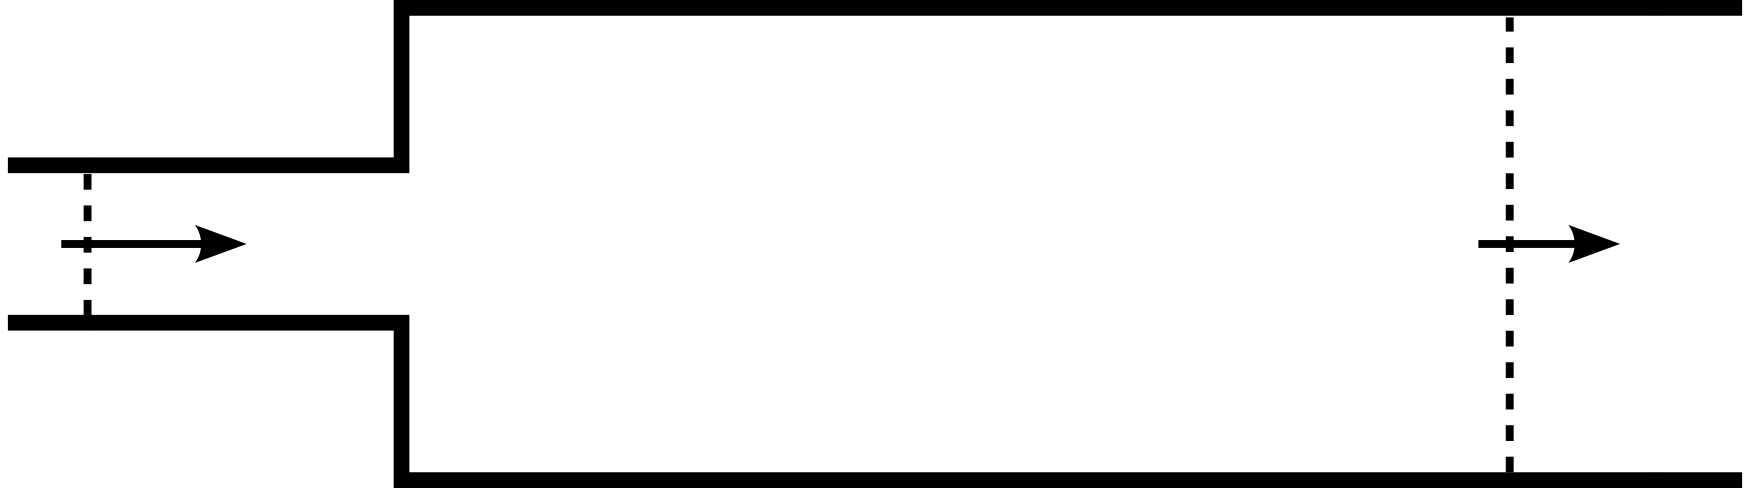
\includegraphics[width=72mm]{elargissement1.png}}
      \put(0, 17){\small $u_1, p_1$}
      \put(92, 17){\small $u_2, p_2$}
      \put(10, 8){\small $S_1$}
      \put(83, 0){\small $S_2$}
      \put(50, 31){\small $\Sigma$}

      \put(117, 5){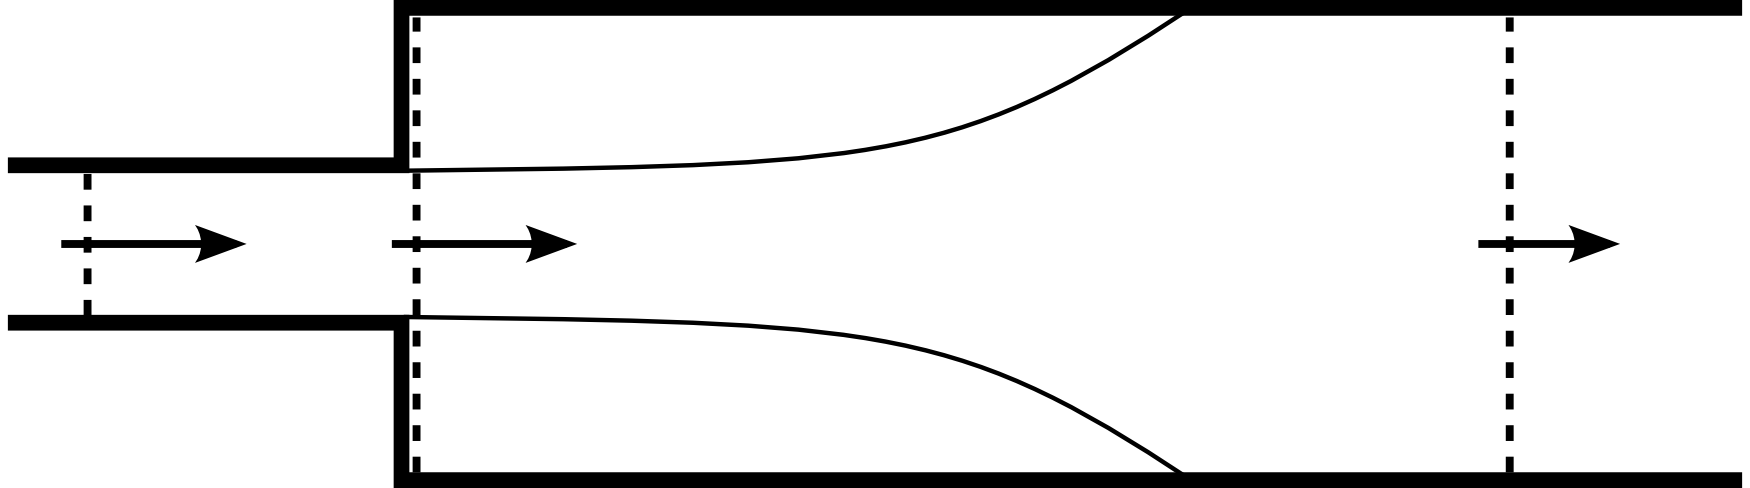
\includegraphics[width=72mm]{elargissement2.png}}
      \put(110, 17){\small $u_1, p_1$}
      \put(148, 17){\small $u_1', p_1'$}
      \put(202, 17){\small $u_2, p_2$}
      \put(120, 8){\small $S_1$}
      \put(137, 0){\small $S_1'$}
      \put(193, 0){\small $S_2$}
      \put(160, 31){\small $\Sigma$}
      \put(141, 25){\small $u \approx 0, p \approx p_1'$}

			\put(50, -4){(a)}
			\put(160, -4){(b)}

   \end{picture}
  \end{center}
  \mycaption{Elargissement brusque dans une conduite : sch\'ema global (a) et d\'etail de l'\'ecoulement d\'ecoll\'e observ\'e exp\'erimentalement (b).}
  \label{fig:elargissement1}
\end{figure}

\begin{enumerate}
\item
  D\'eterminer $u_2$ en fonction de $u_1$ et $s$.
\item
  On n\'eglige dans cette question les effets visqueux et les pertes de charge.
  \begin{enumerate}
  \item
    Quelle quantit\'e physique est conserv\'ee entre les sections $S_1$ et $S_2$ ?
  \item
    En d\'eduire que $p_2 = p_1 + \rho u_1^2 \, f(s)$ o\`u $f(s)$ est à d\'eterminer.
  \item
    En \'ecrivant le bilan int\'egral de quantit\'e de mouvement dans le volume de contrôle
    d\'elimit\'e par la paroi $\Sigma$ de la conduite et les sections $S_1$ et $S_2$,
    montrer que la force exerc\'ee par l'\'ecoulement sur la paroi $\Sigma$ est de la forme
    $F = (S_1 - S_2) \, g(\rho, u_1, p_1, s)$ o\`u $g$ est une fonction à d\'eterminer. 
  \end{enumerate}
\item
  L'exp\'erience montre que la pression $p_2$ pr\'edite pr\'ec\'edemment surestime la r\'ealit\'e
  et que les pertes de charges sont à prendre en compte imp\'erativement après l'\'elargissement.
  En outre, on observe au niveau de l'\'elargissement un d\'ecollement de l'\'ecoulement qui conduit 
  à la formation d'une zone de recirculation dans laquelle la vitesse est n\'egligeable
  (fig.~\ref{fig:elargissement1}b).
  \begin{enumerate}
  \item
    Les pertes de charge restant n\'egligeables entre $S_1$ et la section $S_1'$
    juste après l'\'elargis\-sement, calculer $u_1'$ et $p_1'$.
  \item
    Après l'\'elargissement, on ne peut plus n\'egliger les pertes de charge.
    En consid\'erant le volume de contrôle d\'elimit\'e par les sections dans le fluide $S_1'$
    et $S_2$ et la portion de paroi entre ces deux sections, montrer que 
    $p_2 = p_1 +  \rho u_1^2 \, h(s)$, o\`u $h(s)$ est à d\'eterminer.
  \item
    En d\'eduire que les pertes de charge entre $S_1'$ et $S_2$ s'\'ecrivent
    $\Delta = \rho u_1^2 \,\delta(s)$, o\`u $\delta(s)$ est une fonction à d\'eterminer.
  \item
    Calculer la force exerc\'ee par l'\'ecoulement sur la paroi $\Sigma$ entre $S_1$ et $S_2$.
  \end{enumerate}
\end{enumerate}




%--------------------------------------------------------------------------------------------------
\subsection{Recherche d'un r\'egime d'\'ecoulement \exonormal}
%--------------------------------------------------------------------------------------------------

D\'eterminer le r\'egime d'\'ecoulement (laminaire, turbulent lisse ou turbulent rugueux) 
et le coefficient de perte de charge $\Lambda$ d'un \'ecoulement d'eau 
($\nu = 10^{-6}$ m$^2$/s \`a 15°C) dans les deux cas suivants : 

% \cite[ex. 78]{Com92} :
% \footnote{D'apr\`es Comolet R. 1992 {\it M\'ecanique exp\'erimentale des fluides}, 
% tome 3, exercice 78, Masson.}~:

\begin{enumerate}
\item 
  Tube de verre de diam\`etre $D = 2$ cm et de rugosit\'e $k = 0,2 \mu$m, 
  d\'ebit $Q_v = 0,6$ litre par seconde.
\item 
  Tuyauterie de fonte de diam\`etre $D = 60$ cm et de rugosit\'e $k = 0,3$ mm, 
  d\'ebit $Q_v = 0,85$ m$^3$/s.
\end{enumerate}

On rappelle qu'en \'ecoulement turbulent, le coefficient de perte de charge est donn\'e par 
la formule semi-empirique de Colebrook
$$
  \frac{1}{\sqrt{\Lambda}} = - 2 \log_{10} 
    \left( \frac{k/D}{3,71} + \frac{2,51}{Re \sqrt{\Lambda}} \right).
$$
Une premi\`ere estimation de $\Lambda$ peut \^etre obtenue en ne retenant que le terme dominant 
dans l'argument du logarithme, en consid\'erant que $\Lambda$ est tr\`es g\'en\'eralement compris 
entre 0,01 et 0,04. 
Une deuxi\`eme estimation peut \^etre obtenue en ins\'erant la premi\`ere dans le logarithme, 
et ainsi de suite. 

%--------------------------------------------------------------------------------------------------
\subsection{Ecoulement dans un ol\'eoduc \exonormal}
%--------------------------------------------------------------------------------------------------

On consid\`ere un \'ecoulement d'huile dans un ol\'eoduc horizontal de diam\`etre $D = 10$ cm 
et de longueur $L = 10$ km. 
Le d\'ebit d'huile est $Q_v = 50$ m$^3$/heure, sa densit\'e est $\rho = 950$ kg/m$^3$ 
et de viscosit\'e dynamique $\mu = 0,2$ Pa\,s.

\begin{enumerate}
\item 
  L'\'ecoulement est-il laminaire ou turbulent~? 
  D\'eterminer la perte de charge et le coefficient de perte de charge $\Lambda$.
\item 
  D\'eterminer la puissance dissip\'ee dans la conduite 
  (on pourra utiliser le th\'eor\`eme de l'\'energie cin\'etique).
\item 
  Pour limiter l'\'epaisseur et donc le coût de la conduite, on d\'esire que la pression 
  ne d\'epasse nulle part 5 MPa. Quelle solution peut-on proposer~?
  % \cite[ex. 68]{Com92} 
  % \footnote{D'apr\`es Comolet R. 1992 {\it M\'ecanique exp\'erimentale des fluides}, 
  % tome 3, exercice 68, Masson.}
\end{enumerate}




% !TEX root = TD_fluides_part2_2018.tex

%==================================================================================================
\section{Acoustique}
%==================================================================================================

\setcounter{subsection}{-1}
 
 \subsection{Transmission et réflexion}

{\em exercice préparatoire ; correction sur moodle}

On étudie la transmission et la réflexion d'une onde sonore entre un milieu (1) de masse volumique $\rho_1$ et vitesse du son $c_1$ occupant le demi-espace $x<0$ et un milieu (2) de masse volumique $\rho_2$ et vitesse du son $c_2$ occupant le demi-espace $x>0$.

Une source sonore située dans le milieu (1) et loin de la surface produit une onde progressive monochromatique de la forme $p_+(x,t) = A \cos ( \omega (t-x/c_1)) $. Une partie de l'énergie de l'onde se réfléchit, et une partie est transmise.

\begin{enumerate}

\item 
Justifiez qu'il est légitime de chercher une solution de la forme 
$$
p'(x,t) = A \cos ( \omega (t-x/c_1)) + B \cos ( \omega (t+x/c_1)) \mbox{ pour } x<0 ;
$$
$$
p'(x,t) = C \cos ( \omega (t-x/c_2)) \mbox{ pour } x>0.
$$

\item Donnez la forme du champ de vitesse $u(x,t)$ correspondant.

\item En écrivant la continuité des vitesses et des pressions en $x=0$, calculez le coefficient de réflexion en amplitude $B/A$ et le coefficient de transmission en amplitude $C/A$.

\item En déduire que le coefficient de transmission en intensité acoustique vaut :

$$ 
T_i = \frac{4 \rho_1 c_1 \rho_2 c_2}{(\rho_1 c_1+\rho_2 c_2)^2}
$$

\item Application : calculez le coefficient de transmission entre l'eau et l'air.

\end{enumerate}


 
  
 \subsection{Acoustique des instruments à vent}

Les instruments à vent employés dans l'orchestre sont classiquement regroupés en famille des bois et cuivre selon le mode l'excitation du tuyau par le souffle du musicien (embouchure pour les cuivres, anches ou biseau pour les vents). Cette classification "historique" n'est pas très pertinente 
du point de vue de l'acoustique musicale. De ce point de vue, les propriétés essentielles sont :

\begin{itemize}

\item La forme du résonateur. De ce point de vue on distingue les instruments cylindriques (flûte, clarinette...), les instruments coniques (hautbois, saxophone, ...), et les instruments combinant une section cylindrique et une section conique (trompette, cor, trombone...). 
\footnote{Ajoutons que la présence d'un pavillon n'est pas essentielle à la modélisation acoustique, et qu'il existe aussi des instruments à résonateur globulaire (ocarina) fonctionnant selon le principe du résonnateur de Helmholtz} 

\item Le fait que le tuyau soit ouvert ou fermé en entrée et en sortie. On distingue les instruments ouvert-ouvert (flûte traversière, flûte à bec, tuyaux d'orgue), les instruments ouverts-fermés 
(flûtes de pan) et les instruments fermés-ouverts (tous les instruments à anche ou à embouchure pour lesquels le bec se comporte comme une extrémité fermée).

\end{itemize}

\subsubsection*{A. La Flûte}

On modélise une flûte traversière par un cylindre de longueur $L$ et de rayon $a$, supposé ouvert à ses deux extrémités.

\begin{enumerate}
\item 
Rappelez l'équation de Helmholtz gouvernant la pression acoustique $p'(x,t)$, et la relation entre la pression acoustique et le débit massique $q(x,t)$.

%\item Quelle condition limite faut-il appliquer sur la pression et sur le débit sur une extrémité fermée ?

\item Donnez les conditions limites est vérifiées par $p'$ et $q$ en $x=0$ et $x=L$, en 
supposant qu'aux deux extrémités la pression est égale à la pression atmosphérique (hypothèse d'extrémité {\em idéalement ouverte}).

\item On cherche la solution sous la forme de mode propre (ou onde stationnaire) de la forme 
$p'(x,t) = P(x) \cos (\omega t+ \phi)$. A partir de l'équation de Helmholtz, donnez les valeurs des fréquences et tracez la forme des trois premiers modes propres. A quelles positions sont les noeuds de pression et de débit associés à ces modes ?

\item On considère le mode fondamental (de fréquence la plus basse). Montrez que la structure du mode peut s'écrire sous la forme de deux ondes progressives se propageant en direction opposées. Par un raisonnement simple retrouvez la valeur de la fréquence fondamentale.

\item Application : calculez la fréquence fondamentale (théorique) d'une flûte traversière de 
longueur $66cm$ et d'une clarinette de même longueur.

\item Une modélisation plus poussée de l'écoulement au voisinage des extrémités montre 
que les noeuds de pression sont en réalité situés à une distance $\Delta = 0.85 a$ de chacune des extrémités. Calculez, en pourcentage (puis en demi-tons) la modification de fréquence due à cette correction.

\end{enumerate}


\subsubsection*{B. La clarinette}

On modélise une clarinette par un cylindre de longueur $L$ et de rayon $a$, 
supposé ouvert à la sortie mais fermé à l'entrée.

\begin{enumerate}

\item Donnez, dans ce cas, les conditions limites est vérifiées par $p'$ et $q$ en $x=0$ et $x=L$.

\item En cherchant de nouveau la solution sous la forme de mode propre, 
donnez les valeurs des fréquences et tracez la forme des trois premiers modes propres. A quelles positions sont les noeuds de pression et de débit associés à ces modes ?

\item Comparez la fréquence fondamentale d'une clarinette à celle d'une flûte. Que constate-t-on ? 

\end{enumerate}


\subsubsection*{C. Le hautbois}

Un hautbois peut être modélisé par un tuyau conique de longueur $L$, rayon en sortie $a$
(ce qui correspond à un angle d'ouverture $\alpha = \tan^{-1}( a/L)$), supposé ouvert en sortie et (forcément) fermé en entrée (car terminé par une pointe d'épaisseur nulle...)

\begin{enumerate}

\item Justifiez que la pression doit être cherchée sous la forme $p'(r,t)$ où $r$ est le rayon en coordonnée sphérique.

\item Donnez l'expression de l'équation de Helmholtz en coordonnées sphériques.

\item On cherche de nouveau la solution sous la forme de modes propres. Montrez que ceux-ci sont de la forme $p'(r,t) = A \sin(\omega r/c )/r \cos ( \omega t)$. Quelles sont les fréquences des modes propres ? 

\item Tracez, pour les 3 premiers modes, la forme de la pression $p'(x,t)$ et du 
débit acoustique $q(r,t)$ correspondant. 

\item Comparez la fréquence fondamentale d'un hautbois de longueur $L$ à celles d'une flûte et d'une clarinette de même longueur. Que constate-t-on ?

\end{enumerate}
  


\subsubsection*{D. Le trombone$^*$}

Un trombone peut être modélisé comme un cylindre de longueur $L_2$ et de rayon $a$, fermé en entrée, raccordé à un cône de même longueur $L_1$ et de rayon final $R = 5a$, ouvert en sortie (on ne tient pas compte du pavillon).

\begin{enumerate}

\item Donnez l'angle $\alpha$ du cône et la position théorique de la pointe de celui-ci.
(on note $x_1$ la distance entre la pointe et le raccord entre les deux parties du tuyau).

\item On suppose que dans la section cylindrique la solution prend la forme d'une onde plane ($p' = P(x) \cos \omega t $) et que dans la section conique elle prend la forme d'une onde sphérique 
($p' = Q(r)/r \cos \omega t$). En supposant que la pression et le débit acoustique sont continus au raccord entre les deux sections du tuyau, montrez que les fréquences des modes propres
sont solutions de l'équation suivante :

$$
\tan (k L_2) - \cot (k L_1) - \frac{1}{kx_1} = 0.
$$

\end{enumerate}

\subsubsection*{E. Discussion}

\begin{enumerate}
\item Comparez la fréquence fondamentale d'un hautbois de longueur $L$ à celles d'une flûte et d'une clarinette de même longueur. Que constate-t-on ?

\item Pour des raisons musicales, un instrument de musique a un son harmonieux si les fréquences des modes supérieurs (les partiels) sont multiples de la fréquence du mode fondamental. Cette relation est-elle vérifiée par les instruments considérés dans cet exercice ?


\end{enumerate}

Pour en savoir plus : {\em Acoustics of musical instruments, N. H. Fletcher \& T. D. Rossing}.



%--------------------------------------------------------------------------------------------------
\subsection{R\'esonateur de Helmholtz$^*$}
%--------------------------------------------------------------------------------------------------

En soufflant dans une bouteille, on peut lui faire \'emettre un son. 
Or la fr\'equence de ce son est beaucoup plus basse que ce que donne le calcul simple 
qui consid\`ere que le fond et l'ouverture de la bouteille sont respectivement un n{\oe}ud 
et un ventre de vitesse. 
Ainsi, un frontignan (75 centilitres) \'emet un son voisin du $la_1$ d'un piano, 
soit 110 Hz (essayez !), alors que consid\'erer que la longueur de la bouteille correspond 
\`a $\lambda/4$ donne environ 420 Hz. 
Le probl\`eme g\'en\'eral est celui de la fr\'equence de r\'esonance d'une cavit\'e perc\'ee 
d'un trou.

Helmholtz a r\'esolu le probl\`eme en consid\'erant que l'air dans la cavit\'e (la bouteille) 
se comporte comme un ressort sans masse, auquel est suspendue une  masse d'air cylindrique 
oscillant rigidement au voisinage du trou (dans le goulot). 
Montrer que la fr\'equence de r\'esonance est alors donn\'ee par
$
\omega^2 = c^2 \pi r^2 / (V_0 l),
$
o\`u $c$ est la vitesse du son, $V_0$ est le volume de la cavit\'e, et $l$ et $r$ la longueur 
et le rayon de la masse oscillante. 
Ce mod\`ele donne-t-il le bon r\'esultat pour un frontignan ($V_0$ = 750 cm$^3$, $r = 1$ cm, 
$l = 9$ cm) ? 
(Pour \^etre pr\'ecis, il faut prendre en compte une longueur effective de la masse oscillante, 
somme de la longueur $l_g$ du goulot et de la correction de Rayleigh, \'egale \`a $0,6 \, r$, 
\`a chaque extr\'emit\'e du goulot. 
Une autre complication, plus difficile \`a prendre en compte, provient du fait qu'un frontignan 
n'est pas exactement constitu\'e de deux cylindres.) 

Le mod\`ele de Helmholtz peut \^etre justifi\'e par un bilan de masse dans la cavit\'e 
(o\`u la masse volumique peut \^etre suppos\'ee uniforme puisque la longueur de la cavit\'e 
est petite devant la longueur d'onde), et par un bilan de quantit\'e de mouvement dans le goulot 
(o\`u la vitesse peut \^etre suppos\'ee uniforme pour la m\^eme raison). 
Montrer que ces deux \'equations donnent l'\'equation d'un oscillateur harmonique pour 
les variations de masse volumique dans la cavit\'e, dont la pulsation propre est donn\'ee 
par l'\'equation ci-dessus.






% !TEX root = TD_fluides_part2_2018.tex


\setcounter{section}{10}


\section{Ecoulements compressibles}


%--------------------------------------------------------------------------------------------------
\subsection{Limite de l'hypoth\`ese incompressible}
%--------------------------------------------------------------------------------------------------

Un tube de Pitot double est plac\'e sur l'axe d'une canalisation de 10 cm
de diam\`etre contenant de l'air en \'ecoulement.
Le manom\`etre diff\'erentiel en U du tube de Pitot est rempli de mercure
de masse volumique $\rho_{Hg}$ = 13 600 kg.m$^{-3}$.
\begin{enumerate}
\item
Quel est le d\'ebit d'air obtenu dans l'hypoth\`ese d'un \'ecoulement
incompressible sachant que la d\'enivellation $\Delta h$ du mercure est
de 10 mm ?
\item
En consid\'erant que les effets de compressibilit\'e peuvent \^etre
n\'eglig\'ees pour des fluctuations de masse volumique de l'air $\rho$
inf\'erieures \`a 1\%,
jusqu'\`a quel nombre de Mach l'\'ecoulement peut \^etre consid\'er\'e
comme incompressible~?
Quelle est alors l'erreur commise sur l'\'evaluation de la vitesse ?
\end{enumerate}

%--------------------------------------------------------------------------------------------------
\subsection{Vol subsonique}
%--------------------------------------------------------------------------------------------------

Un avion vole \`a un nombre de Mach de 0.95 \`a une altitude o\`u la pression
atmosph\'erique est \'egale \`a 0.223 bar et o\`u la masse volumique de l'air
est $\rho=0.349$ kg.m$^{-3}$.
On suppose que l'air se comporte comme un fluide parfait et que les filets
fluides sont thermiquement isol\'es.
\begin{enumerate}
\item
Calculer la vitesse de l'avion en km/h.
\item
Calculer la pression et la temp\'erature au point d'arr\^et sur le bord
d'attaque de l'aile.
\end{enumerate}
 
%--------------------------------------------------------------------------------------------------
\subsection{Ecoulement isentropique}
%--------------------------------------------------------------------------------------------------

Dans un turbo-r\'eacteur, les gaz entrent dans la tuy\`ere \`a la vitesse
de 275 m.s$^{-1}$ et \`a une temp\'erature de 741 $^o$C.
Leur vitesse de sortie est de 564 m.s$^{-1}$.
En supposant le fluide parfait et l'\'ecoulement isentropique, calculer
\begin{enumerate}
\item
la temp\'erature de sortie des gaz,
\item
le nombre de Mach dans les conditions d'\'ejection des gaz.
\end{enumerate}
On assimilera les gaz \`a de l'air pur ($C_p = 1000$ J.kg$^{-1}$.K$^{-1}$).

%--------------------------------------------------------------------------------------------------
\subsection{R\'egimes isentropiques dans une tuyère}
%--------------------------------------------------------------------------------------------------

On consid\`ere dans ce probl\`eme l'\'ecoulement isentropique
d'un gaz parfait dans une tuy\`ere
intercal\'ee entre un r\'eservoir \`a air comprim\'e et l'atmosph\`ere
\`a pression $P_a = 1$ atm.
On assimilera le gaz \`a de l'air pur ($\gamma = 1.405$, 
$r=287$ J/kg/K).
La section de sortie a un diam\`etre $D_s = 5$ cm.

\begin{enumerate}
\setcounter{enumi}{0}
\item[]
\textbf{R\'egime 1 :}
\item[]
Dans ce r\'egime, la vitesse du gaz au niveau du col de la tuy\`ere
est $u_c = 250$ m/s.
La temp\'erature dans le r\'eservoir est $T_i = 300$ K.
\item
Calculer la temp\'erature au col $T_c$
puis le nombre de Mach au col $M_c$.
\item
En d\'eduire la nature (subsonique, supersonique ou sonique)
de l'\'ecoulement dans le convergent, au col et dans le divergent.
\item
\label{it:T_ext}
Par continuit\'e, la temp\'erature en sortie de la tuy\`ere est \'egale
\`a la temp\'erature ext\'erieure ambiante $T_s = T_a = 296$ K.
Calculer le nombre de Mach $M_s$ dans la section de sortie.
\item
\label{it:P_ext}
De la m\^eme fa\c{c}on, la pression en sortie de tuy\`ere $P_s$ correspond
\`a la pression atmosph\'erique $P_a$.
En d\'eduire la pression g\'en\'eratrice $P_i$ dans le r\'eservoir
puis la masse volumique g\'en\'eratrice $\rho_i$.
\item
Calculer la vitesse en sortie $u_s$ et la masse volumique en sortie $\rho_s$
puis en d\'eduire le d\'ebit massique $\dot{m}$ de la tuy\`ere.
\item[]
\textbf{R\'egime 2 :}
\item[]
Dans cette partie, la pression $P_i$ dans le r\'eservoir est augment\'ee
jusqu'\`a ce que le nombre de Mach en sortie atteigne $M_s = 1.5$.
Pour ce r\'egime, on observe ni onde de choc ni onde de d\'etente~:
la tuy\`ere est dite \textit{adapt\'ee}.
\item
D\'eterminer la nature (subsonique, supersonique ou sonique)
de l'\'ecoulement dans le convergent, au col et dans le divergent.
\item
Les conditions thermodynamiques en sortie de tuy\`ere sont les m\^emes
que dans les questions \ref{it:T_ext} et \ref{it:P_ext}.
En d\'eduire la pression g\'en\'eratrice $P_i$ et la temp\'erature
g\'en\'eratrice $T_i$ r\'egnant dans le r\'eservoir \`a air comprim\'e.
\item
	Calculer la temp\'erature au col $T_c$.
\item
	Calculer le diam\`etre de la section au col $D_c$.
\item
	Calculer le d\'ebit massique $\dot{m}$ pour ce r\'egime de fonctionnement de la tuy\`ere.
\end{enumerate}

%==================================================================================================
%\section{Ondes de choc}
%==================================================================================================

% !TEX root = TD_fluides_part2_2018.tex



\setcounter{section}{11}

\section{Ondes de choc}


%--------------------------------------------------------------------------------------------------
\subsection{Tube de Pitot en \'ecoulement supersonique}
%--------------------------------------------------------------------------------------------------

On considère un \'ecoulement supersonique uniforme dont on cherche à mesurer les caract\'eristiques
(vitesse $u_1$, nombre de Mach $M_1$, pression $p_1$, pression g\'en\'eratrice $p_{i1}$) 
à l'aide d'un tube de Pitot double.
\begin{enumerate}
\item
D\'ecrire qualitativement l'\'ecoulement dans le voisinage du tube de Pitot.
\item
D\'eterminer l'expression du nombre de Mach $M_2$ au niveau du tube de Pitot en fonction
des pressions $p_2$ et $p_{i2}$ mesur\'ees par le tube de Pitot.
\item
En d\'eduire $M_1$.
\item
D\'eterminer $p_1$ et $p_{i1}$.
\item
Expliquer comment il serait possible de pr\'edire la vitesse $u_1$ de l'\'ecoulement incident. 
\end{enumerate}
 
%--------------------------------------------------------------------------------------------------
\subsection{R\'egime d'\'ecoulement discontinu dans une tuyère}
%--------------------------------------------------------------------------------------------------

On considère un \'ecoulement dans une tuyère caract\'eris\'e par la pr\'esence d'une onde de choc.
On souhaite d\'ecrire ce r\'egime particulier de fonctionnement de la tuyère.   
\begin{enumerate}
\item
Pr\'eciser dans quelle partie de la tuyère se trouve cette onde de choc.
Peut-il exister une autre onde de choc dans la tuyère ?
\item
Donner le nombre de Mach au col $M_c$.
\item
Tracer pour un tel r\'egime l'allure de la vitesse, de la pression et du nombre de Mach
le long de la tuyère.
\item
Que devient l'onde de choc lorsque la pression en sortie $p_s$ diminue ?
\item 
D\'eterminer en fonction des conditions g\'en\'eratrices en amont la plage
de pression $p_s$ correspondant à ce r\'egime d'\'ecoulement discontinu dans la tuyère.
\end{enumerate}
 
%--------------------------------------------------------------------------------------------------
\subsection{Onde de choc dans une tuyère}
%--------------------------------------------------------------------------------------------------

Une tuyère convergente-divergente est aliment\'ee avec de l'air à pression
g\'en\'eratrice $p_i$ de 3 bars et une temp\'erature $T_i$ de 600 K.
Cette tuyère a une section d'entr\'ee $A_e$ de 5 cm$^2$ dans laquelle la vitesse
$u_e$ a pour valeur 146 m.s$^{-1}$.
On constate lors du fonctionnement la pr\'esence d'une onde de choc dans
la section $A\indice{choc}$ d'aire 2.53 cm$^2$.
L'objectif de cet exercice est d'utiliser les relations isentropiques et de saut afin
de d\'eterminer certaines caract\'eristiques de l'\'ecoulement \'etudi\'e.
\begin{enumerate}
\item
  Calculer la pression $p_c$, la temp\'erature $T_c$ et la masse volumique $\rho_c$ au col ainsi
  que le d\'ebit massique $\dot{m}$ de la tuyère.
\item
  Calculer les pressions $p_1$ et $p_2$ et les temp\'eratures $T_1$ et $T_2$
  imm\'ediatement en amont et en aval de l'onde de choc.
\item
  Calculer la pression $p_s$ et la temp\'erature $T_s$ dans la section de sortie $A_s$ d'aire
  2.70 cm$^2$.
\end{enumerate}

 
 
 
 
% !TEX root = TD_fluides_part2_2018.tex

\section{Ecoulements Inertiels I : bilans intégraux}

%% !TEX root = TD_fluides_part2_2018.tex

%\appendix












%\pause

%\addcontentsline{toc}{section}{B. Diagramme de Moody}
\clearpage
\section{Pertes de charges et Diagramme de Moody}
$$
\Delta P = \frac{\rho U^2 L}{D} \lambda(Re,\epsilon)
$$

$$ 
Re = \frac{U D}{\nu}, \quad \epsilon = \frac{k}{D}
$$

\begin{description}
\item[Régime laminaire ($Re \leq 2000$) ]
$$
\lambda = \frac{64}{Re}
$$
\item[Régime turbulent  ($Re \geq 2000$) ]

Pour $\varepsilon < 0.01\%$ et $Re<10^5$ on peut utiliser  la formule de Blasius
\begin{equation}
   \lambda= 0.316 \, Re^{-1/4}
 \end{equation}

Pour $Re >4000$ et $\epsilon$ quelconque, on utilise généralement la formule de Colebrook (semi-explicite) :
\begin{equation}
  \frac{1}{\sqrt{\lambda}} = -2 \log_{10} \left (
  \frac{2.51}{Re\sqrt{\lambda}} + \frac{\varepsilon}{3.71}
  \right)
\end{equation}
\end{description}



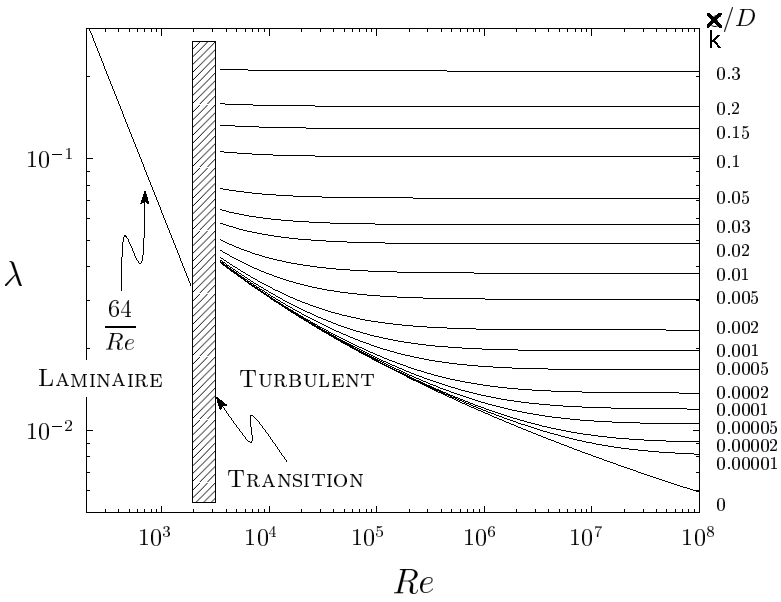
\includegraphics[width=\linewidth]{Moody_diagram.pdf}


\addcontentsline{toc}{section}{C. Ecoulement compressible isentropique de gaz parfait}
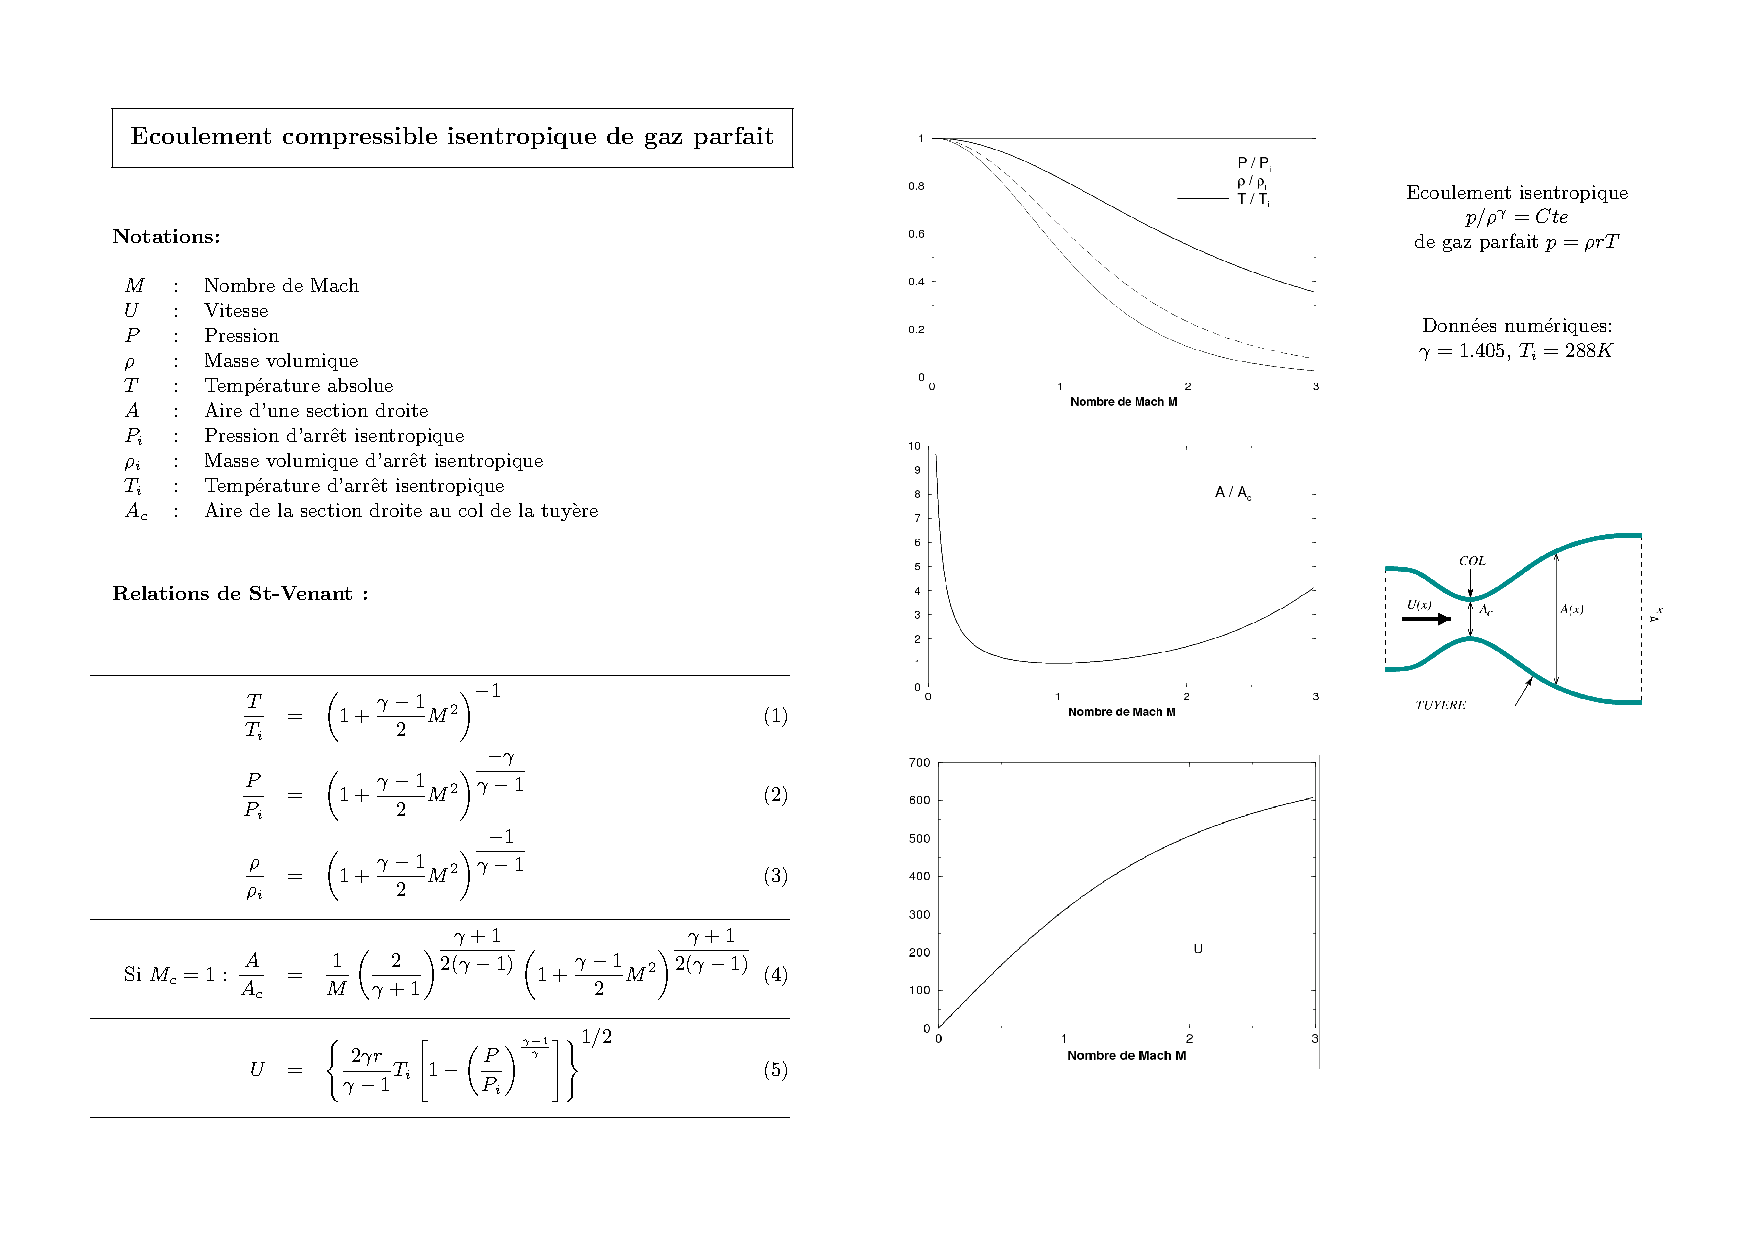
\includepdf[pages=1-2, landscape]{./Figures/St_Venant.pdf}

\addcontentsline{toc}{section}{D. Relations de saut a travers un choc droit}
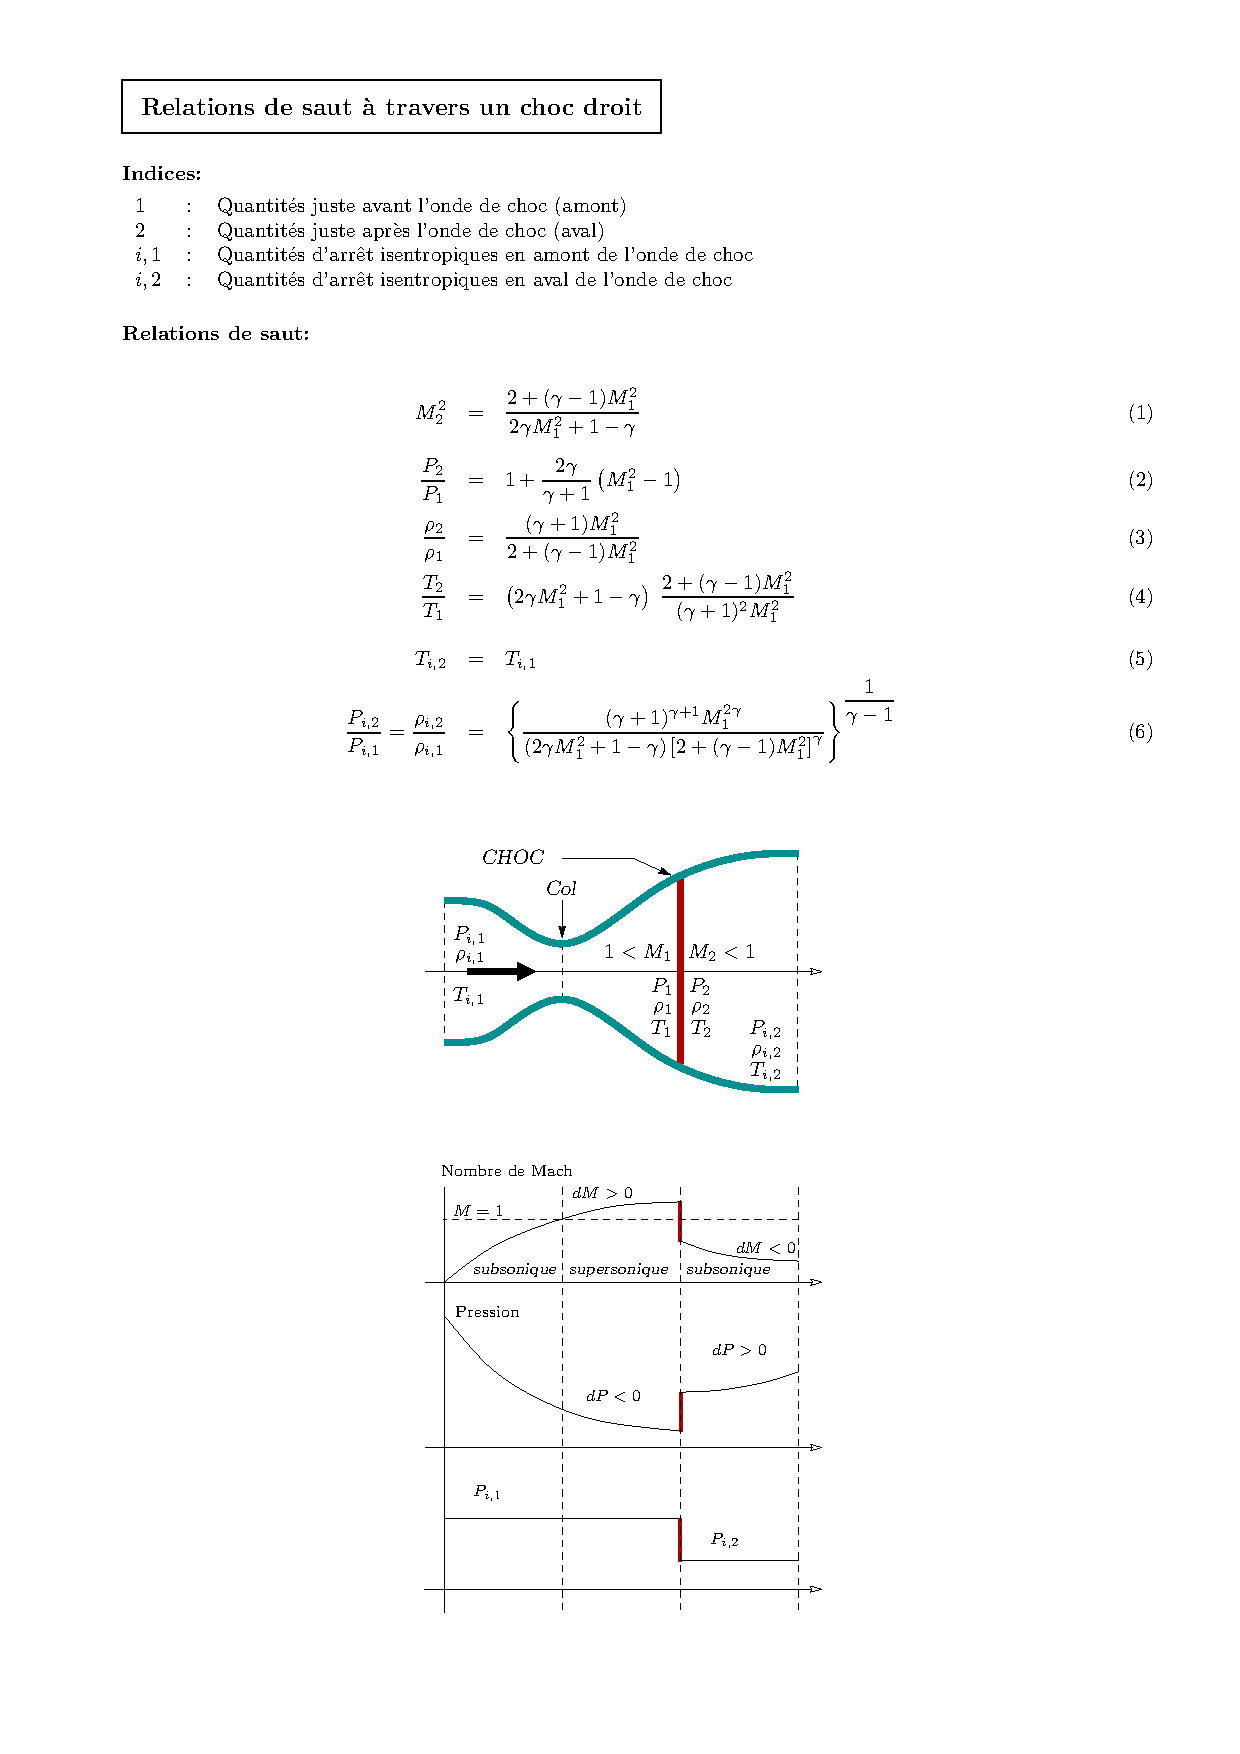
\includepdf[pages=1-2]{./Figures/choc.pdf}



\end{document}





